\documentclass[11pt,a4paper,titlepage]{article}
\usepackage[english, ngerman]{babel}
%\usepackage{bibgerm} % Zum Einbinden einer Bibliothek (wird hier nicht benötigt)
\usepackage[latin1]{inputenc}
\usepackage{graphicx}
\usepackage{epstopdf} % wandelt automatisch eps- in pdf-Dateien um, falls pdf als Ausgabeformat gewählt wird
\usepackage{include/IHA_listing} % einbinden von Quellcode
\setupListingMatlab % lade Setup für Matlab Quellcode, Parameter können in der *.sty file geändert werden ;)
\usepackage[top=3cm, bottom=2.7cm, left=3cm, right=3cm]{geometry} % Package zum einfachen Einstellen des Seitenlayouts
\usepackage{amsmath} % Package zum Einbinden von Formeln etc.
\usepackage{subfigure}
\usepackage{placeins}
\usepackage{latexsym}
\usepackage{amsfonts}
\usepackage{amssymb}	
\usepackage{fancyhdr}
\usepackage{lastpage}
\usepackage[ngerman, num]{isodate}
\usepackage{marvosym}
\usepackage{eurosym}
\usepackage{url}
\usepackage{wrapfig}
\usepackage{xcolor}
\usepackage{tcolorbox}
\usepackage{hyperref}
\usepackage{tabularx}
\usepackage{enumitem}

\newcommand\ClrSquare[1]{\textcolor{#1}{\rule{7pt}{7pt}}}
\newcommand\ClrSquareBig[1]{\textcolor{#1}{\rule{10pt}{10pt}}}

\parindent0mm
%\usepackage[protrusion=true,expansion=true]{microtype}
%\usepackage[final]{microtype}
%\usepackage{fontspec}
\usepackage{cmbright}


\usepackage{listings}

\usepackage{color}
\definecolor{gray}{rgb}{0.4,0.4,0.4}
\definecolor{darkblue}{rgb}{0.0,0.0,0.6}
\definecolor{cyan}{rgb}{0.0,0.6,0.6}
\definecolor{jadeRed}{rgb}{0.7578, 0.0625, 0.1641}

\definecolor{ml_charging}{rgb}{0, 0.447, 0.741}
\definecolor{ml_error}{rgb}{0.85, 0.325, 0.098}
\definecolor{ml_proposing}{rgb}{0.929, 0.694, 0.125}
\definecolor{ml_connecting}{rgb}{0.494, 0.184, 0.556}
\definecolor{ml_running}{rgb}{0.466, 0.674, 0.188}
\definecolor{ml_quest}{rgb}{0.301, 0.745, 0.933}
\definecolor{ml_offline}{rgb}{0.7, 0.7, 0.7}

\lstset{
  basicstyle=\ttfamily,
  columns=fullflexible,
  showstringspaces=false,
  commentstyle=\color{gray}\upshape,
	numbers=none
}

\lstdefinelanguage{XML}
{
  morestring=[b]",
  morestring=[s]{>}{<},
  morecomment=[s]{<?}{?>},
  stringstyle=\color{black},
  identifierstyle=\color{darkblue},
  keywordstyle=\color{cyan},
  morekeywords={xmlns,version,type}% list your attributes here
}


\tcbset{
    frame code={}
    %center title,
    left=2pt,
    right=0pt,
    top=2pt,
    bottom=0pt,
    %colback=gray!70,
    %%colframe=white,
    %%width=\dimexpr\textwidth\relax,
    enlarge left by=0mm,
    %boxsep=5pt,
    arc=0pt,outer arc=0pt,
    }
\tcbset{before upper={\parindent0em}}

\newcommand{\titleFull}{olMEGA Mobile Software}
\renewcommand{\title}{olMEGA Mobile Software}
\newcommand{\Institute}{Institute of Hearing Technology and Audiology, Oldenburg}
\newcommand{\version}{v2.0}
%
\pagestyle{fancy}
\lhead{\footnotesize \parbox{11cm}{\Institute} }
\rhead{\footnotesize \sffamily \title\ \thepage\ / \pageref{LastPage}}
\lfoot{\footnotesize \parbox{11cm}{Contact: \Letter\ ulrik.kowalk@jade-hs.de} }
\cfoot{}
\rfoot{\footnotesize \sffamily \title\ \thepage\ / \pageref{LastPage}}
\renewcommand{\footrulewidth}{0.4pt}

%
\begin{document} 
 \selectlanguage{english}
\pagestyle{empty}

\sffamily
\mdseries


\textcolor[rgb]{1,1,1}{.}
	\vspace{3cm}
	\begin{center}
	
	\begin{figure}[h]
		\centering
			\includegraphics[width=0.30\textwidth]{images/Logo.jpg}
	\end{figure}
	\vspace{3cm}
	\Huge
	\titleFull \ \version
	\normalsize
	\\
	\vspace{1cm}
	Handbook\\
	\vspace{1cm}
	Last updated: \today\\
	\vspace{1cm}
	Source: \url{https://github.com/ol-MEGA/olMEGA_MobileSoftware.git}
	\vfill
	\end{center}

%
%\cfoot{}
\clearpage

\tableofcontents

\clearpage

\setcounter{page}{1}
\pagestyle{fancy}

\section{Introduction}

The application you have obtained is a version of the olMEGA EMA system. For standalone use no additional equipment will be required except for a computer to facilitate installation and data transfer. The software has been tested on numerous devices running Android versions 9 or later, but is still undergoing development. Please feel free to report bugs or contact us in case of difficulties during installation or usage. The given directions in the operating system settings may vary across devices.


\section{Installation}


\subsection{Requirements}

The device should be reset to its operating system default (\textit{Settings}$\rightarrow$\textit{Backup\&reset}$\rightarrow$\textit{Factory data reset}) prior to the installation. All accounts (\textit{Settings}$\rightarrow$\textit{Accounts}) as well as device administrators (\textit{Settings}$\rightarrow$\textit{Security}$\rightarrow$\textit{Device administrators}) need to be removed, too. On an average size display a \textit{Medium} font size is sufficient (\textit{Settings}$\rightarrow$\textit{Display}$\rightarrow$\textit{Font size}). Required for the installation are:

\begin{itemize}[label=\ClrSquare{jadeRed}]
	\item USB connection between smartphone and computer
	\item Free software \textit{ADB} (Android Debug Bridge), e.g. ``Minimal ADB and Fastboot''
	\item olMEGA mobile .apk installation file
	\item Questionnaire .xml file
	\item Helpful: free Android file manager, e.g. \href{https://total-commander.de.uptodown.com/android}{``Total Commander''} installed on the device
\end{itemize}


\subsection{Installation steps}\label{sub:installation}

\begin{enumerate}

\vspace{0.5cm}

	\item Install ADB on the computer and add it to the system path.\\
	 
	\item Enable the developer options on the smartphone. How to do this might vary from model to model. The usual procedure is by opening \textit{Settings$\rightarrow$About phone}. At the bottom is an entry showing the \textit{Build number}. This needs to be clicked 7 times until a message appears. If not, please consult the search engine of your choice.\\
	
	\item Go to \textit{Settings}$\rightarrow$\textit{Developer options} and enable \textit{USB Debugging}.\\
	
	\item Connect the phone to the computer and allow debugging via the dialogue on the phone.\\
	
	\item The next step is to establish a working connection between the smartphone and the computer. In order to check for a connection, open a console and type\\
	\\
	\colorbox{black!10}{\texttt{adb devices}}.\\
	\\
	If everything is okay, ADB should find a device. If not, check your connection. In case the computer does not understand the command, ADB needs to be added to the system path.\\
	
	\item Now that a connection has been verified, navigate via the console to the directory that holds the .apk file and input\\
	\\
	\colorbox{black!10}{\texttt{adb install olMEGA\_Mobile.apk}}.\\
	\\
	This will install the application. In case an older version of the application is already installed, type\\
	\\
	\colorbox{black!10}{\texttt{adb install-r olMEGA\_Mobile.apk}}.\\
	
	\item In order to make the application a device owner, which is needed for it to run as a dedicated device, type\\
	\\
	\colorbox{black!10}{\texttt{adb shell dpm set-device-owner com.fragtest.android.pa/.AdminReceiver}}.\\
	
	\item On opening, please grant the application permission to record audio as well as memory access. You will be informed that no questionnaire file is present. To copy the questionnaire .xml file to its directory on the smartphone, please enter one of the two the following command from the directory that holds the .xml file ([*].xml is the name of your questionnaire):\\
	\\
	Android version $<$11:\\
	\colorbox{black!10}{\texttt{adb push [*].xml sdcard/olMEGA/quest}}\\
	\\
	Android version 11+:\\
	\colorbox{black!10}{\texttt{adb push [*].xml sdcard/Android/data/com.iha.olmega\_mobilesoftware\_v2/files/quest}}\\
	
\end{enumerate}

\newpage

\section{Using the application}\label{sec_usage}


\subsection{General purpose}

\begin{wrapfigure}{r}{5cm}
\vspace{-0.5cm}
		\centering
			\begin{minipage}{0.30\textwidth}
			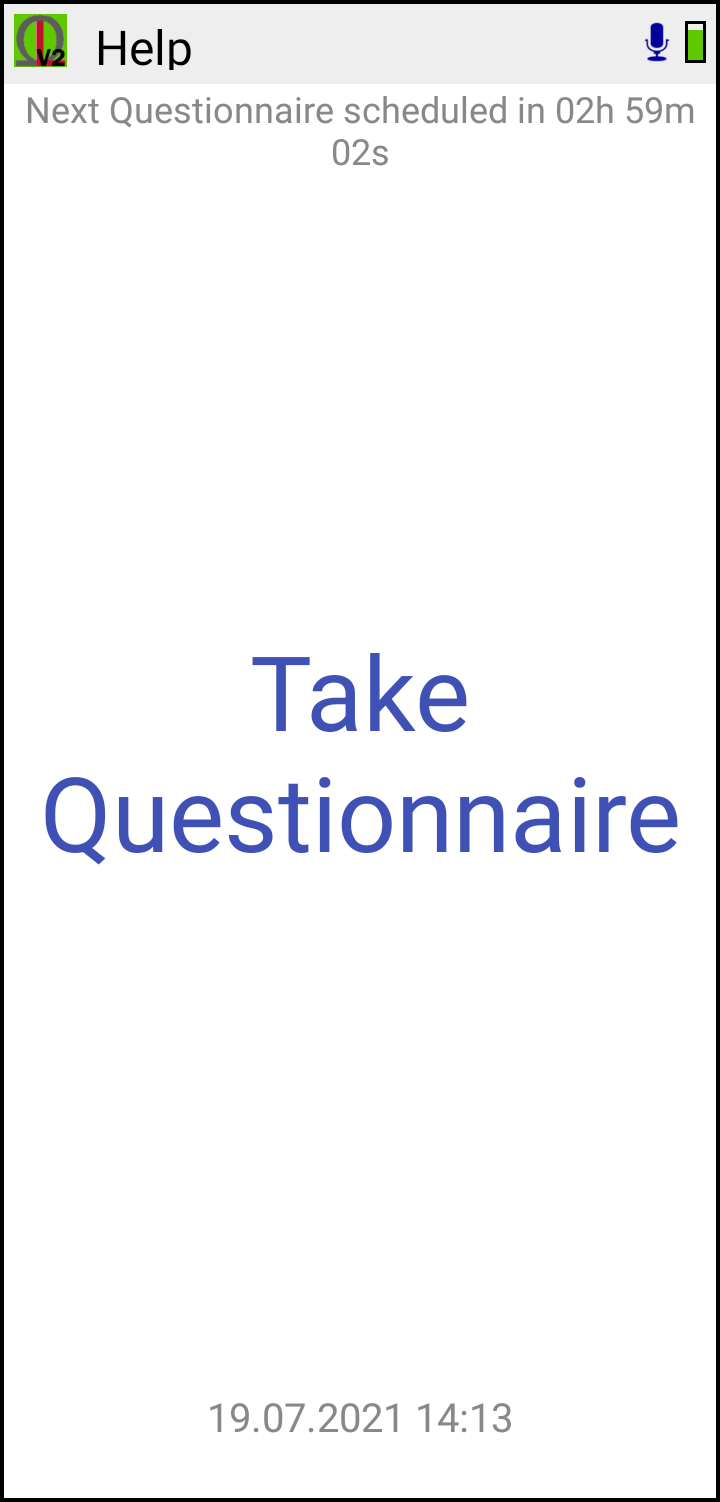
\includegraphics[width=1.00\textwidth]{images/v2_screen_main_ed.png}
			\label{fig:menu}
			\end{minipage}
	\end{wrapfigure}

The main view (see figure on the right) of the application features a bar at the top with a ``Help'' button, providing a general explanation of the main answer formats. Top right are a microphone symbol indicating that the application is running without errors (see also \ref{sub:operationmode}) and a battery symbol displaying the current state of charge.\\
\\
The center of the screen features the ``Take Questionnaire'' button (in case of no major errors present) which can be used to manually start a questionnaire at any given time. Above it is a display of the time until the next questionnaire notification is triggered. If a questionnaire is prompted the font colour changes to red, accompanied by vibrating alert.



\subsection{Configuration Mode}\label{sub:experimenter}

When testing a new questionnaire, it is helpful to disable the Kiosk mode and enable the Configuration mode. Both can be set via the internal preferences menu (\ref{sub:preferences}). Once it is enabled, the logo will turn green (as shown on the screen on the right). You are now free to enter the preferences simply by tapping the logo. 


\subsection{Operation Modes}\label{sub:operationmode}

The olMEGA application comes with 3 pre-configured modes of operation which serve as a starting point as they may be tailored to the experimenter's demands. These operation modes are defined in separate *.xml files that are found in the \texttt{AFEx} folder inside the main application directory. A mode is selected via the preferences menu. Factory presets are:

\begin{itemize}[label=\ClrSquare{jadeRed}]
	\item \texttt{example\_mic\_in\_speaker\_out}: The internal microphone serves as input audio source and the incoming signal is routed to the dynamic acoustic feature extraction stage and from there to the system output. (Warning: This may lead to acoustic feedback.)
	\item \texttt{example\_rfcomm\_in\_audio\_out}: Audio input is received through a serial bluetooth connection via an RFCOMM protocol and fed to a feature extraction engine and finally to the system output. (Warning: This may lead to acoustic feedback.)
	\item \texttt{standalone}: No acoustic data is recorded or extracted.
\end{itemize}

In case of a bluetooth connection, the devices must be paired. More information is provided in \ref{sub:linkdevice}. If either the connection is working fine or no connection is needed (e.g. Standalone mode), the microphone symbol is blue \includegraphics[width=0.02\textwidth]{images/mic_darkblue.png}. In case the application experiences an error significant enough to compromise its functionality, the symbol is greyed out \includegraphics[width=0.02\textwidth]{images/mic_gray.png}.




\subsection{The Preferences Menu}\label{sub:preferences}

The in-app settings can be accessed in two ways. If the ``Configuration Mode'' has been enabled, a short click on the logo icon in the top left corner of the application opens the settings screen. In normal use, a long click of 5 seconds is necessary to access the menu. Here is a list of all available settings:
\begin{center}
\begin{tcolorbox}[colback=black!10!white,colframe=black!50!white, boxsep=1pt,left=4pt,right=14pt,top=4pt,bottom=2pt]
\begin{itemize}[label=\ClrSquare{jadeRed}]
	\item Autostart: If enabled, the app starts automatically.
	\item USB cuts Connection: The bluetooth connection is terminated if a USB connection is made. 
	\item Kiosk Mode: If all prerequisites are met, a KIOSK mode is instantiated, granting the application full control of the device.
	\item Operation Mode: Here the operation mode is selected (see \ref{sub:operationmode})
	\item Use Questionnaire: Determines whether a questionnaire is used
	\item Select Questionnaire: Click to select a questionnaire from a list 
	\item Show Countdown: If enabled, a countdown until the next alarm is displayed. 
	\item ClientID: If an external (i.e. web-based) questionnaire is used, this is the id used to register
	\item Link Device: Use this function to link a bluetooth device 
	\item Version: Shows the current version number
	\item Configuration Mode: If enabled, the user can access the settings quickly and may exit questionnaires by clicking on the green logo in the top left corner. (see \ref{sub:experimenter})
	\item Kill App and Service: The most reliable way to shut down the application. If KIOSK mode is active, it is also the only way (that does not include hacking).
	\item Unset Device Admin: This deprives the application of its special privileges and is needed only before uninstalling. 
	\item Check for Update: This option guides the user through an automated update process. The user is notified if additional permissions are necessary.
\end{itemize}
\end{tcolorbox}
\end{center}




\subsection{Languages}

The application currently supports English, German, and Swedish. Language settings are adjusted automatically, according to the language setting of the smartphone.


\subsection{Log}


A log file named ``\textit{log.txt}''is created in the main directory that includes information which can be used to understand and retrace the behavior of the application. 

\newpage

\begin{wrapfigure}{r}{5cm}
\vspace{-0.5cm}
		\centering
			\begin{minipage}{0.30\textwidth}
			\includegraphics[width=1.00\textwidth]{images/linking.png}
			\label{fig:menu}
			\vspace{-2cm}
			\end{minipage}
	\end{wrapfigure}

\subsection{Link Device}\label{sub:linkdevice}

Linking a transmitter to the smartphone is mandatory if a bluetooth source is used as audio input for acoustical features. An integrated linking process makes this step very simple and the user is guided by on-screen information (see image on the right). Access to the process is gathered through the in-app settings. Firstly the transmitter is powered on. Then, the button ``Link transmitter'' is pressed. Once a connection has been established, the window may be closed.



\section{Compilation of a questionnaire}


\subsection{General outline}

The questionnaires are generated on the basis of .xml files which can be altered to suit the needs of the experiment. Generally it is a good idea to start from an existing file and make changes, testing them regularly on the smartphone in order to guarantee errorless functionality. In case of formal mistakes (e.g. missing brackets or typos within tags) the application might crash. 


\subsection{Location of questionnaire files}

Questionnaire files are placed in the \texttt{quest} folder located inside the main directory. The application will automatically sort all questionnaire files alphabetically and pick the uppermost. If you would like to use a specific questionnaire, you can choose manually from the preferences menu (see \ref{sub:experimenter}), but we recommend placing only a single file in the \texttt{quest} folder in order to avoid confusion. 


\subsection{Head}

The head consists of two lines that must not be changed, but may become obsolete in future releases.

\begin{center}
\begin{tcolorbox}[colback=black!10!white,colframe=black!50!white, boxsep=1pt,left=4pt,right=4pt,top=4pt,bottom=2pt]
\texttt{<?xml version="1.0" encoding="utf-8"?>\\
<mobiquest>}
\end{tcolorbox}
\end{center}


\subsection{Timer}

Two different timer settings exist: \textit{interval} and \textit{fixed schedule}. When choosing interval, a \texttt{mean} and \texttt{deviation} value can be set. The application generates a random interval true to a uniform distribution within the given limits (mean$\pm$deviation). This can be beneficial in order to avoid sampling artifacts, e.g. suggesting a questionnaire every 60 minutes to someone who is always listening to the news at that time. If the scheduling interval should not be random, a deviation value of "0" is set. The timer is re-initiated after a questionnaire has been finalized.

\begin{center}
\begin{tcolorbox}[colback=black!10!white,colframe=black!50!white, boxsep=1pt,left=4pt,right=4pt,top=4pt,bottom=2pt]
\texttt{<timer mean="1800" deviation="300"></timer>}
\end{tcolorbox}
\end{center}

If it is desired to suggest a questionnaire at specific times during the day, the \texttt{date} value must be set. The value is entered in form of a String, meaning a time within quotation marks, e.g. "13:47". The system uses the 24h format HH:mm and multiple dates can be entered by concatenating times with a semicolon, e.g. "12:15;17:21;14:41". Times are sorted automatically by the application. 

\begin{center}
\begin{tcolorbox}[colback=black!10!white,colframe=black!50!white, boxsep=1pt,left=4pt,right=4pt,top=4pt,bottom=2pt]
\texttt{<timer date="12:15;13:13;14:41;17:21;08:10;08:12"></timer>}
\end{tcolorbox}
\end{center}


\subsection{Title}

The title tag can be set to personal taste and is formally needed but does not appear in the output result files.

\begin{center}
\begin{tcolorbox}[colback=black!10!white,colframe=black!50!white, boxsep=1pt,left=4pt,right=4pt,top=4pt,bottom=2pt]
\texttt{<title>\\
\hspace*{0.5cm}<text>Exemplary Questionnaire</text>\\
</title>}
\end{tcolorbox}
\end{center}


\subsection{Questions}

A question consists of an opening \texttt{question} tag including some properties, e.g. id, type, and filter. Then follows the label -- the actual question. After that usually comes a suite of answer options, which are defined by a unique \texttt{option id}. Although there are no restrictions, it has proven useful in practice to concatenate \texttt{question id} and \# of the answer option using an underscore (the underscore is omitted internally) as question ID. Since, internally, questions are sorted by ascending ID, a meaningful sequence is advisable. The question ID serves as a unique question identifier and the \texttt{type} sets the answer format. There are seven different formats available.


\subsubsection{Single Choice: Radio buttons}

Radio buttons are established as single choice option symbols, meaning that only one option can be selected at the same time.

\begin{center}
\hspace{-1.1cm}
	\begin{tabular}{p{0.68\textwidth} p{0.25\textwidth}} 
		\raisebox{-\totalheight}{
		\begin{tcolorbox}[colback=black!10!white,colframe=black!50!white, boxsep=1pt,left=4pt,right=4pt,top=4pt,bottom=2pt]
		\texttt{\noindent
					$<$question id="10101" type="radio"$>$\newline
					\hspace*{0.5cm}$<$\textbf{label}$>$\newline
					\hspace*{1cm}$<$text$>$Which record is the best?$<$/text$>$\newline
					\hspace*{0.5cm}$<$/\textbf{label}$>$\newline
					\hspace*{0.5cm}$<$\textbf{option} id="10101\_01"$>$\newline
					\hspace*{1cm}$<$text$>$Dark side of the moon$<$/text$>$\newline
					\hspace*{0.5cm}$<$/\textbf{option}$>$\newline
					\hspace*{0.5cm}$<$\textbf{option} id="10101\_02"$>$\newline
					\hspace*{1cm}$<$text$>$Grand Tour$<$/text$>$\newline
					\hspace*{0.5cm}$<$/\textbf{option}$>$\newline
					\hspace*{0.5cm}$<$\textbf{option} id="10101\_03"$>$\newline
					\hspace*{1cm}$<$text$>$Foxtrot$<$/text$>$\newline
					\hspace*{0.5cm}$<$/\textbf{option}$>$\newline
					$<$/\textbf{question}$>$
					}
			\end{tcolorbox} 
		}
		&
		\vspace{-0.29cm}
		\raisebox{-\totalheight}{
			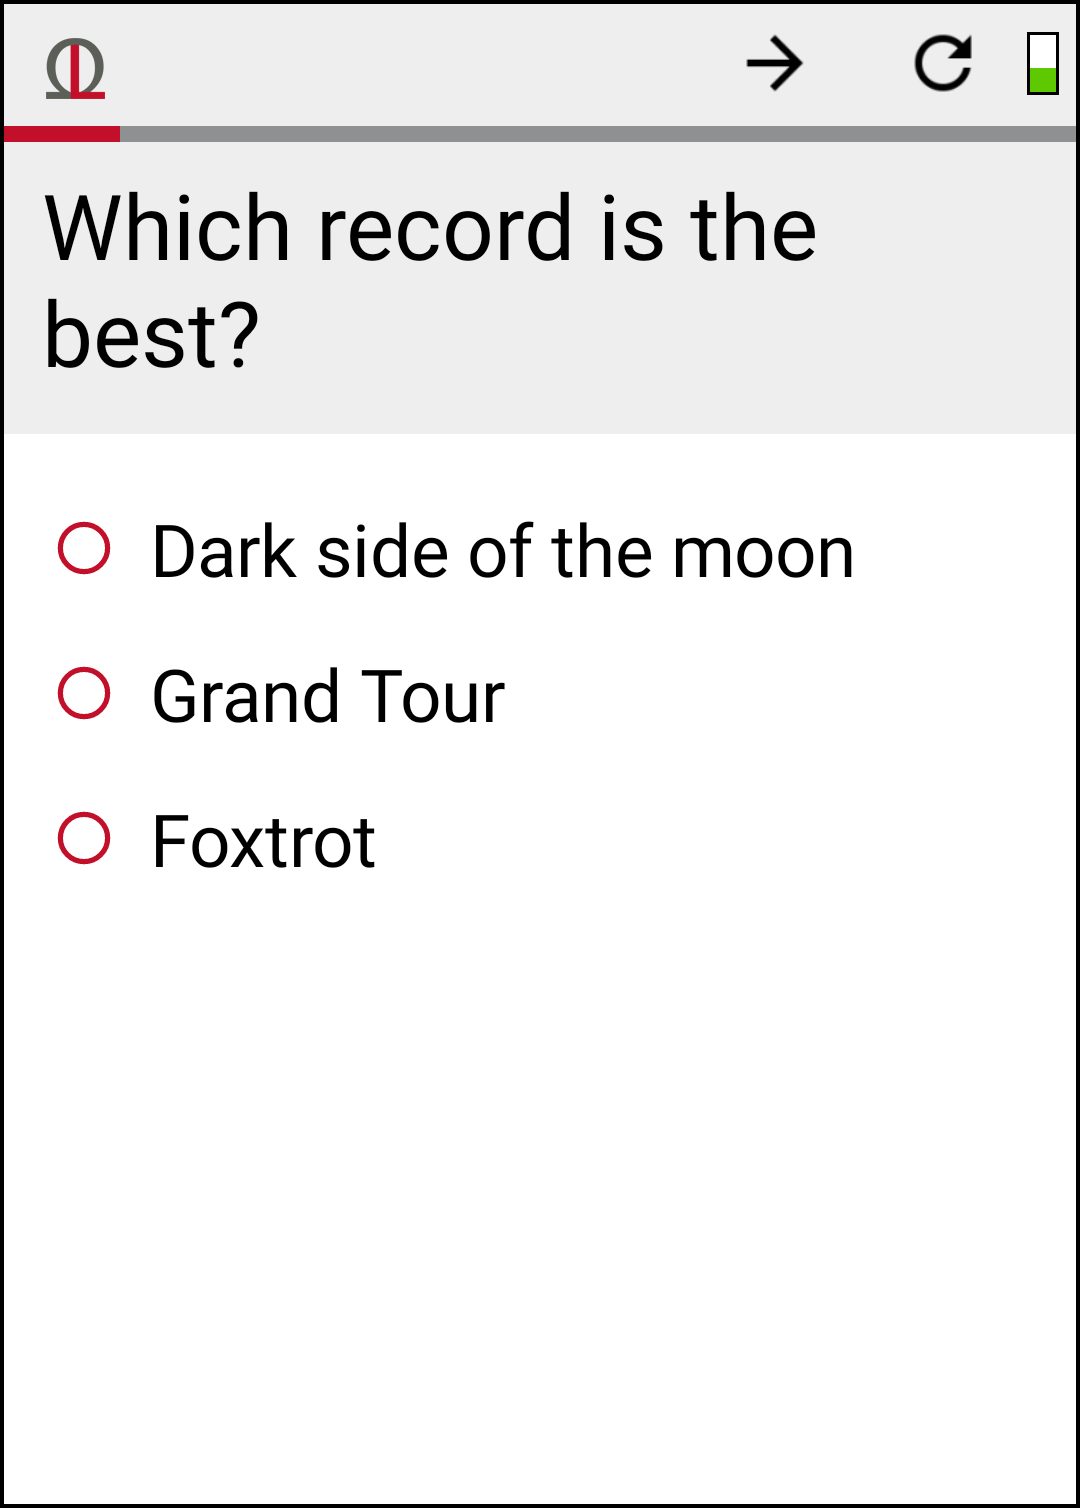
\includegraphics[width=0.30\textwidth]{images/screen_radio_crop_box.png}
		}
	\end{tabular}\\
\end{center}


\subsubsection{Multiple Choice: Checkboxes}

Checkboxes give the user the impression of a list from which multiple items can be selected at the same time. Customized within-list logic can be implemented as described in \ref{subsec:goupingandexclusivity}. 

\begin{center}
\hspace{-1.1cm}
	\begin{tabular}{p{0.68\textwidth} p{0.25\textwidth}} 
		\raisebox{-\totalheight}{
		\begin{tcolorbox}[colback=black!10!white,colframe=black!50!white, boxsep=1pt,left=4pt,right=4pt,top=4pt,bottom=2pt]
		\texttt{\noindent
				$<$question id="10102" type="checkbox"$>$\newline
				\hspace*{0.5cm}$<$label$>$\newline
				\hspace*{1.0cm}$<$text$>$Please select one or more.$<$/text$>$\newline
				\hspace*{0.5cm}$<$/label$>$\newline
				\hspace*{0.5cm}$<$option id="10102\_01"$>$\newline
				\hspace*{1.0cm}$<$text>Red$<$/text$>$\newline
				\hspace*{0.5cm}$<$/option$>$\newline
				\hspace*{0.5cm}$<$option id="10102\_02"$>$\newline
				\hspace*{1.0cm}$<$text$>$Green$<$/text$>$\newline
				\hspace*{0.5cm}$<$/option$>$\newline
				\hspace*{0.5cm}$<$option id="10102\_03"$>$\newline
				\hspace*{1.0cm}$<$text$>$Blue$<$/text$>$\newline
				\hspace*{0.5cm}$<$/option$>$\newline
				</question>
				}
		\end{tcolorbox} 
		}
		&
		\vspace{-0.29cm}
		\raisebox{-\totalheight}{
			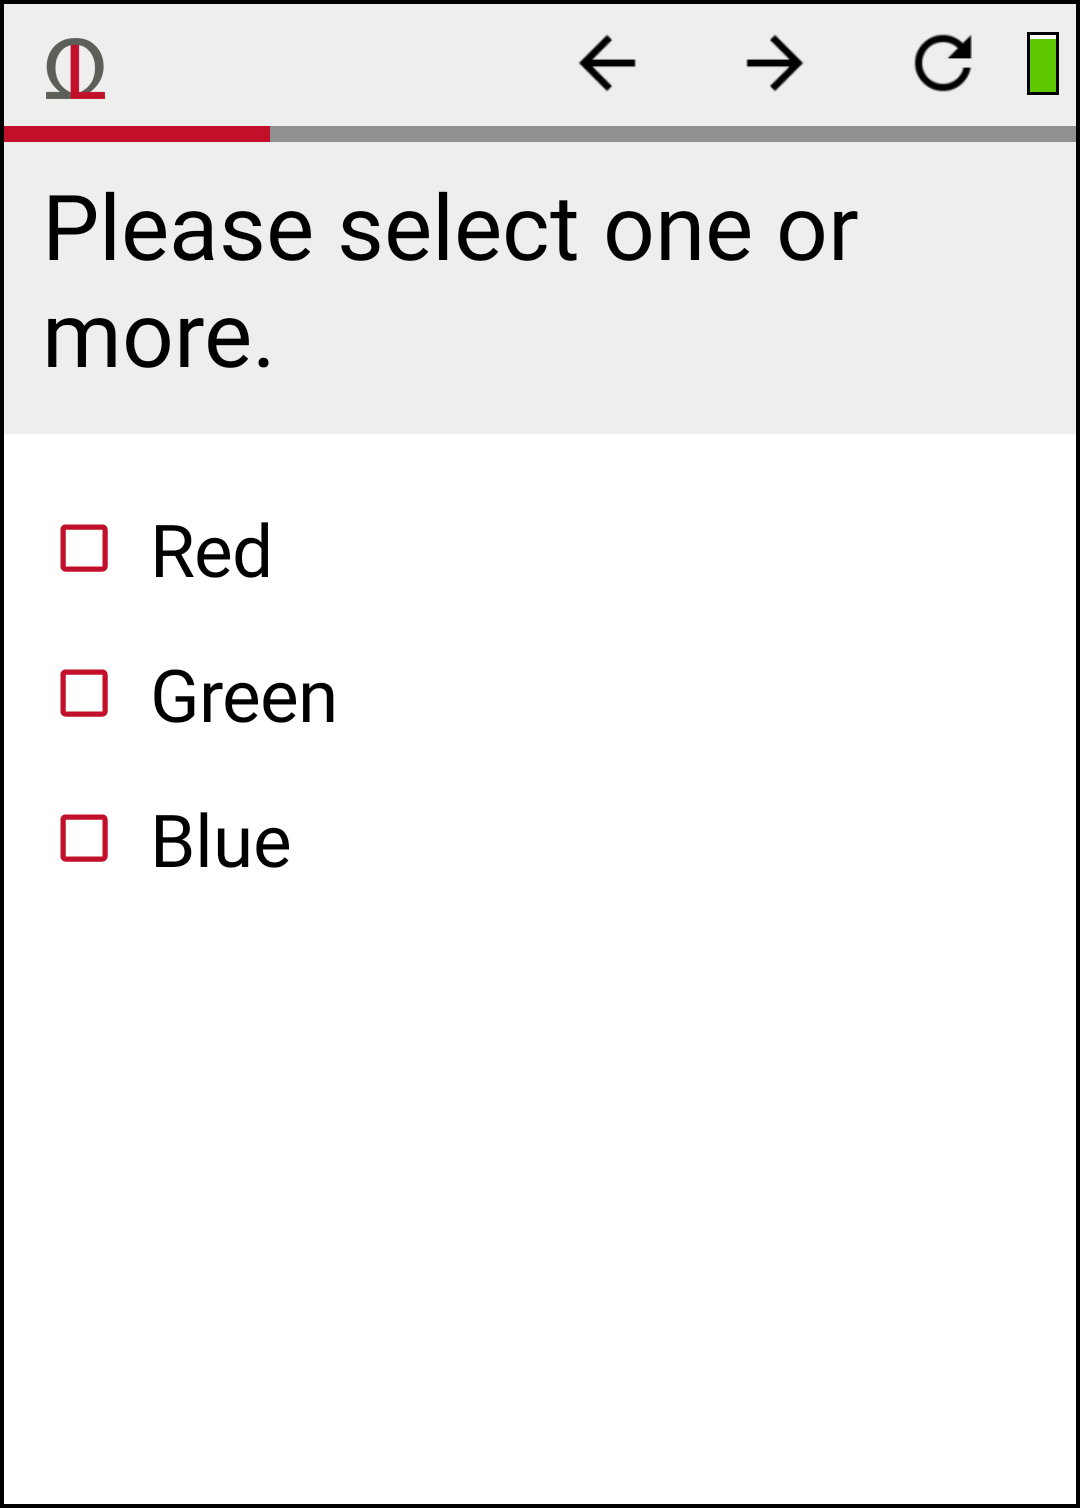
\includegraphics[width=0.30\textwidth]{images/screen_checkbox_crop_box.png}
		}
	\end{tabular}\\
\end{center}




\subsubsection{Emojis}  

Emojis yield a swift and intuitive way of assessing the emotional state of a subject. The application comes with five built-in emojis, which are called directly via their file names as shown below. 

\begin{center}
\hspace{-1.1cm}
	\begin{tabular}{p{0.68\textwidth} p{0.25\textwidth}} 
		\raisebox{-\totalheight}{
		\begin{tcolorbox}[colback=black!10!white,colframe=black!50!white, boxsep=1pt,left=4pt,right=4pt,top=4pt,bottom=2pt]
		\texttt{\noindent
			$<$question id="10103" type="emoji"$>$\newline
			\hspace*{0.5cm}$<$label$>$\newline
			\hspace*{1.0cm}$<$text$>$How are you feeling?$<$/text$>$\newline
			\hspace*{0.5cm}$<$/label$>$\newline
			\hspace*{0.5cm}$<$option id="10103\_01"$>$\newline
			\hspace*{1.0cm}$<$text$>$emoji\_happy2$<$/text$>$\newline
			\hspace*{0.5cm}$<$/option$>$\newline
			\hspace*{0.5cm}$<$option id="10103\_02"$>$\newline
			\hspace*{1.0cm}$<$text$>$emoji\_happy1$<$/text$>$\newline
			\hspace*{0.5cm}$<$/option$>$\newline
			\hspace*{0.5cm}$<$option id="10103\_03"$>$\newline
			\hspace*{1.0cm}$<$text$>$emoji\_neutral$<$/text$>$\newline
			\hspace*{0.5cm}$<$/option$>$\newline
			\hspace*{0.5cm}$<$option id="10103\_04"$>$\newline
			\hspace*{1.0cm}$<$text$>$emoji\_sad1$<$/text$>$\newline
			\hspace*{0.5cm}$<$/option$>$\newline
			\hspace*{0.5cm}$<$option id="10103\_05"$>$\newline
			\hspace*{1.0cm}$<$text$>$emoji\_sad2$<$/text$>$\newline
			\hspace*{0.5cm}$<$/option$>$\newline
			$<$/question$>$
			}
		\end{tcolorbox} 
		}
		&
		\vspace{-0.29cm}
		\raisebox{-\totalheight}{
			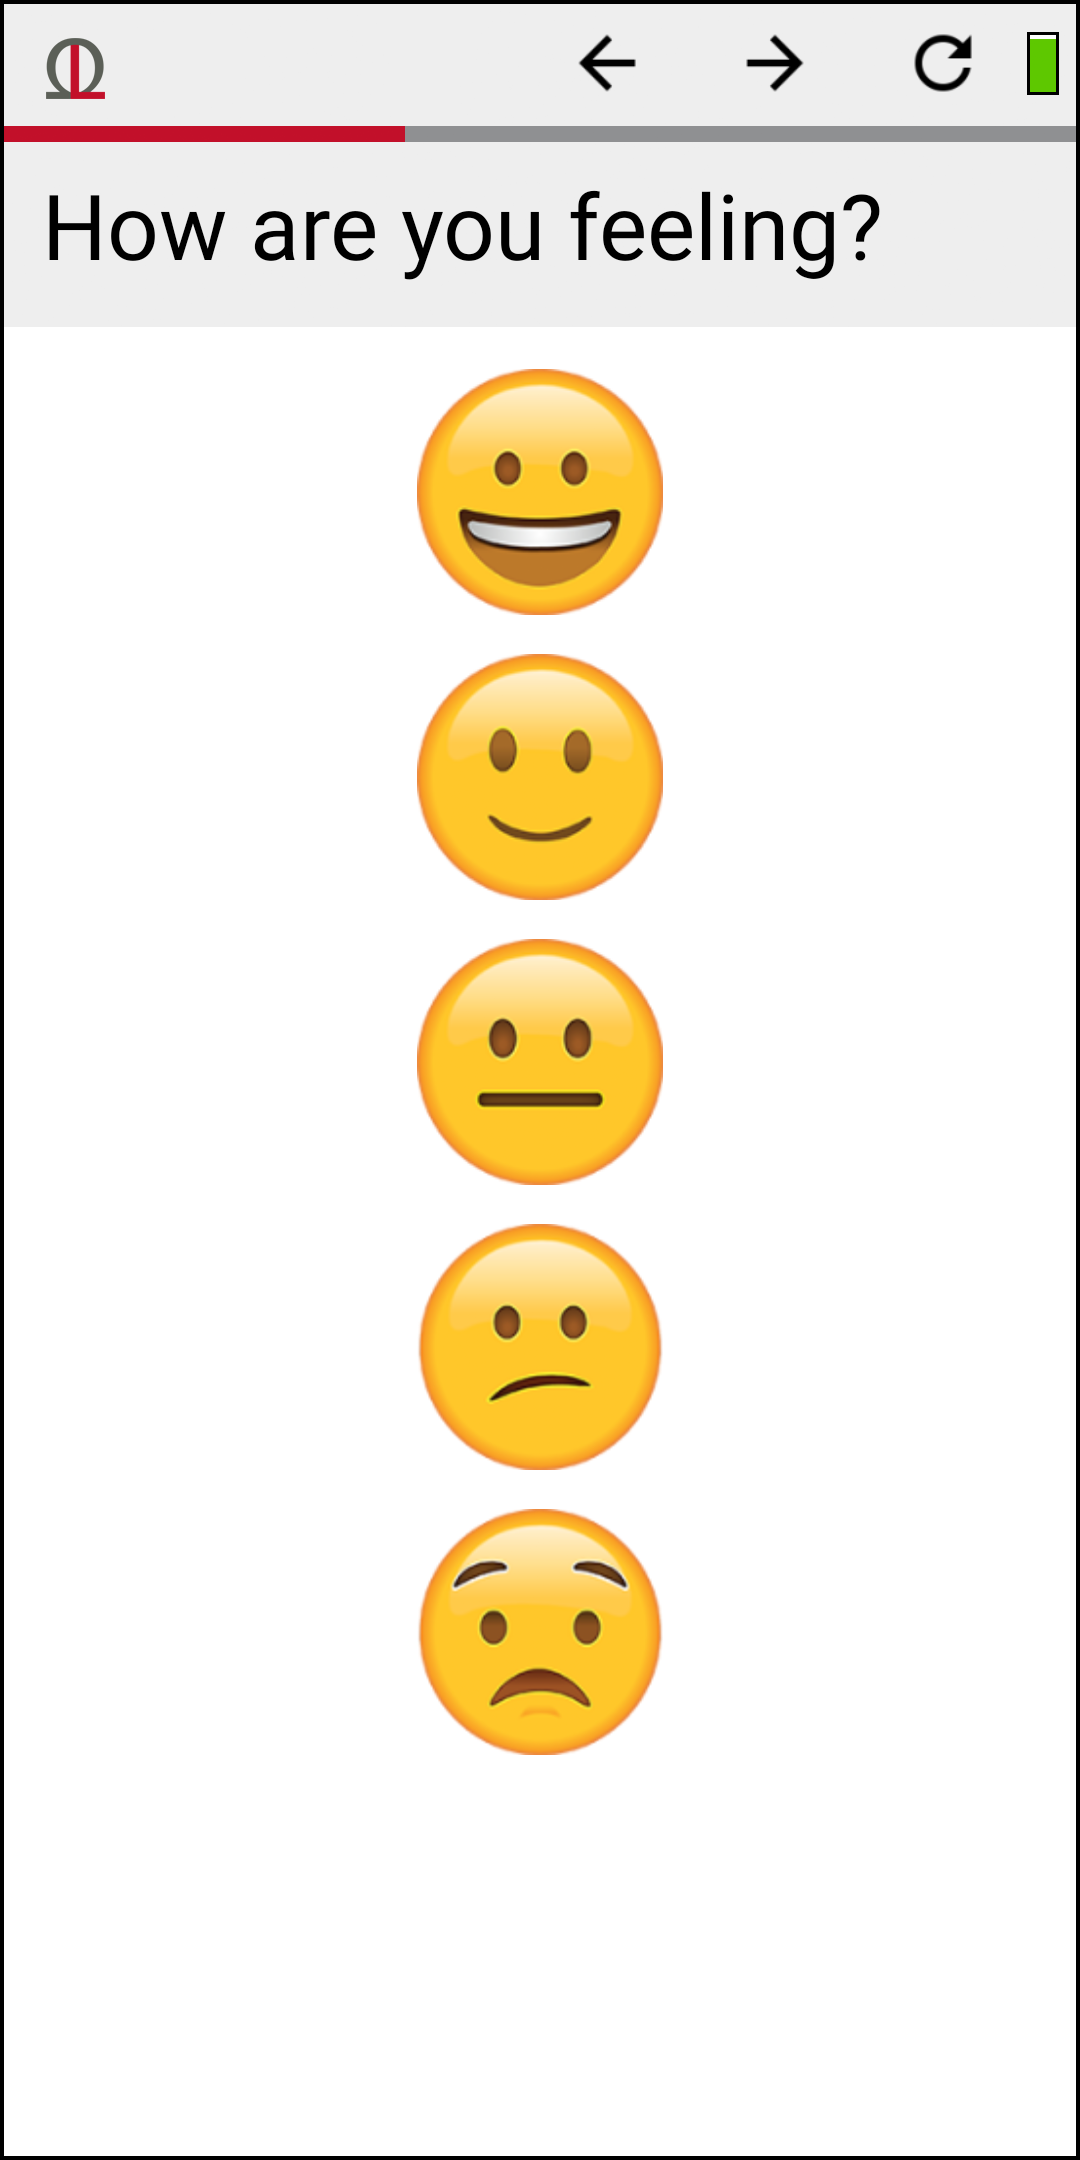
\includegraphics[width=0.30\textwidth]{images/screen_emoji_box.png}
		}
	\end{tabular}\\
\end{center}


\newpage

\subsubsection{Text}

Sometimes the best way of assessing a situation is to have the user enter a short text. 

\begin{center}
\hspace{-1.1cm}
	\begin{tabular}{p{0.68\textwidth} p{0.25\textwidth}} 
		\raisebox{-\totalheight}{
		\begin{tcolorbox}[colback=black!10!white,colframe=black!50!white, boxsep=1pt,left=4pt,right=4pt,top=4pt,bottom=2pt]
		\texttt{\noindent
			$<$question id="10104" type="text"$>$\newline
			\hspace*{0.5cm}$<$label$>$\newline
			\hspace*{1.0cm}$<$text$>$Please enter text.$<$/text$>$\newline
			\hspace*{0.5cm}$<$/label$>$\newline
			$<$/question$>$
			}
		\end{tcolorbox} 
		}
		&
		\vspace{-0.29cm}
		\raisebox{-\totalheight}{
			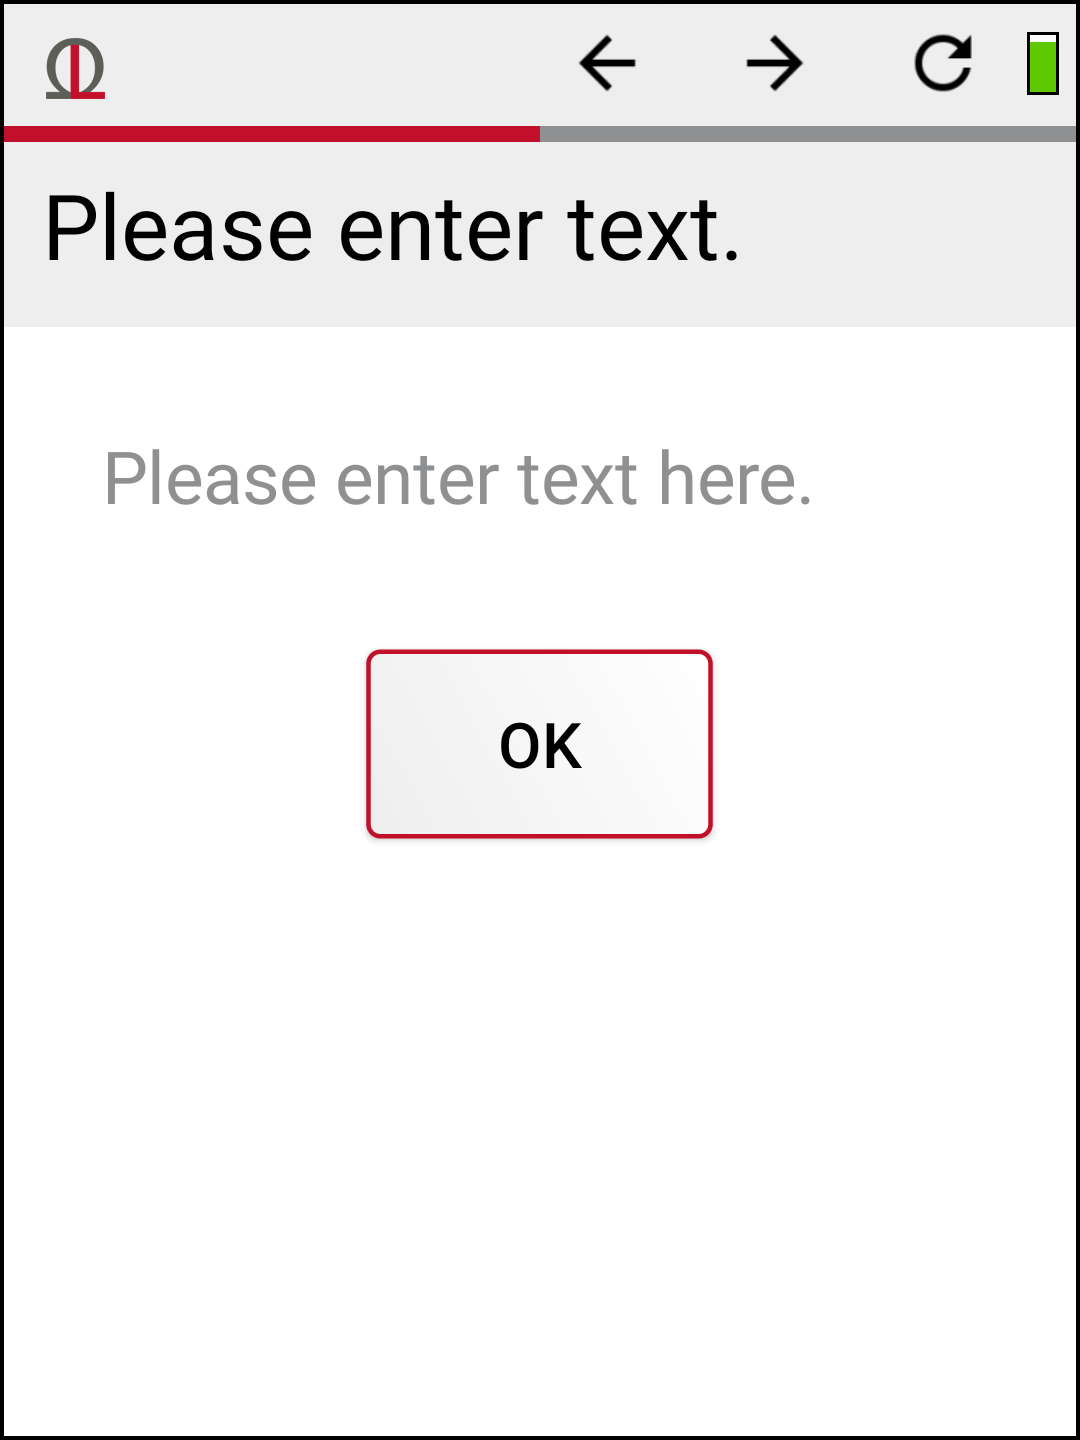
\includegraphics[width=0.30\textwidth]{images/screen_text_crop_box.png}
		}
	\end{tabular}\\
\end{center}


\subsubsection{Fixed Slider}

Fixed sliders technically do not offer a different choice than radio buttons, but they can be helpful when the answer has a sense of level to it. The slider will snap to the nearest position, alternatively the categories are selectable themselves.

\begin{center}
\hspace{-1.1cm}
	\begin{tabular}{p{0.68\textwidth} p{0.25\textwidth}} 
		\raisebox{-\totalheight}{
		\begin{tcolorbox}[colback=black!10!white,colframe=black!50!white, boxsep=1pt,left=4pt,right=4pt,top=4pt,bottom=2pt]
		\texttt{\noindent
			$<$question id="10105" type="sliderFix"$>$\newline
			\hspace*{0.5cm}$<$label$>$\newline
			\hspace*{1.0cm}$<$text>How loud is it?$<$/text$>$\newline
			\hspace*{0.5cm}$<$/label$>$\newline
			\hspace*{0.5cm}$<$option id="10105\_01"$>$\newline
			\hspace*{1.0cm}$<$text$>$Very loud$<$/text$>$\newline
			\hspace*{0.5cm}$<$/option$>$\newline
			\hspace*{0.5cm}$<$option id="10105\_02"$>$\newline
			\hspace*{1.0cm}$<$text>Loud$<$/text$>$\newline
			\hspace*{0.5cm}$<$/option$>$\newline
			\hspace*{0.5cm}$<$option id="10105\_03"$>$\newline
			\hspace*{1.0cm}$<$text>Medium$<$/text$>$\newline
			\hspace*{0.5cm}$<$/option$>$\newline
			\hspace*{0.5cm}$<$option id="10105\_04"$>$\newline
			\hspace*{1.0cm}$<$text$>$Not loud$<$/text$>$\newline
			\hspace*{0.5cm}$<$/option$>$\newline
			\hspace*{0.5cm}$<$option id="10105\_05"$>$\newline
			\hspace*{1.0cm}$<$text>Quiet$<$/text$>$\newline
			\hspace*{0.5cm}$<$/option$>$\newline
			$<$/question$>$
			}
		\end{tcolorbox} 
		}
		&
		\vspace{-0.29cm}
		\raisebox{-\totalheight}{
			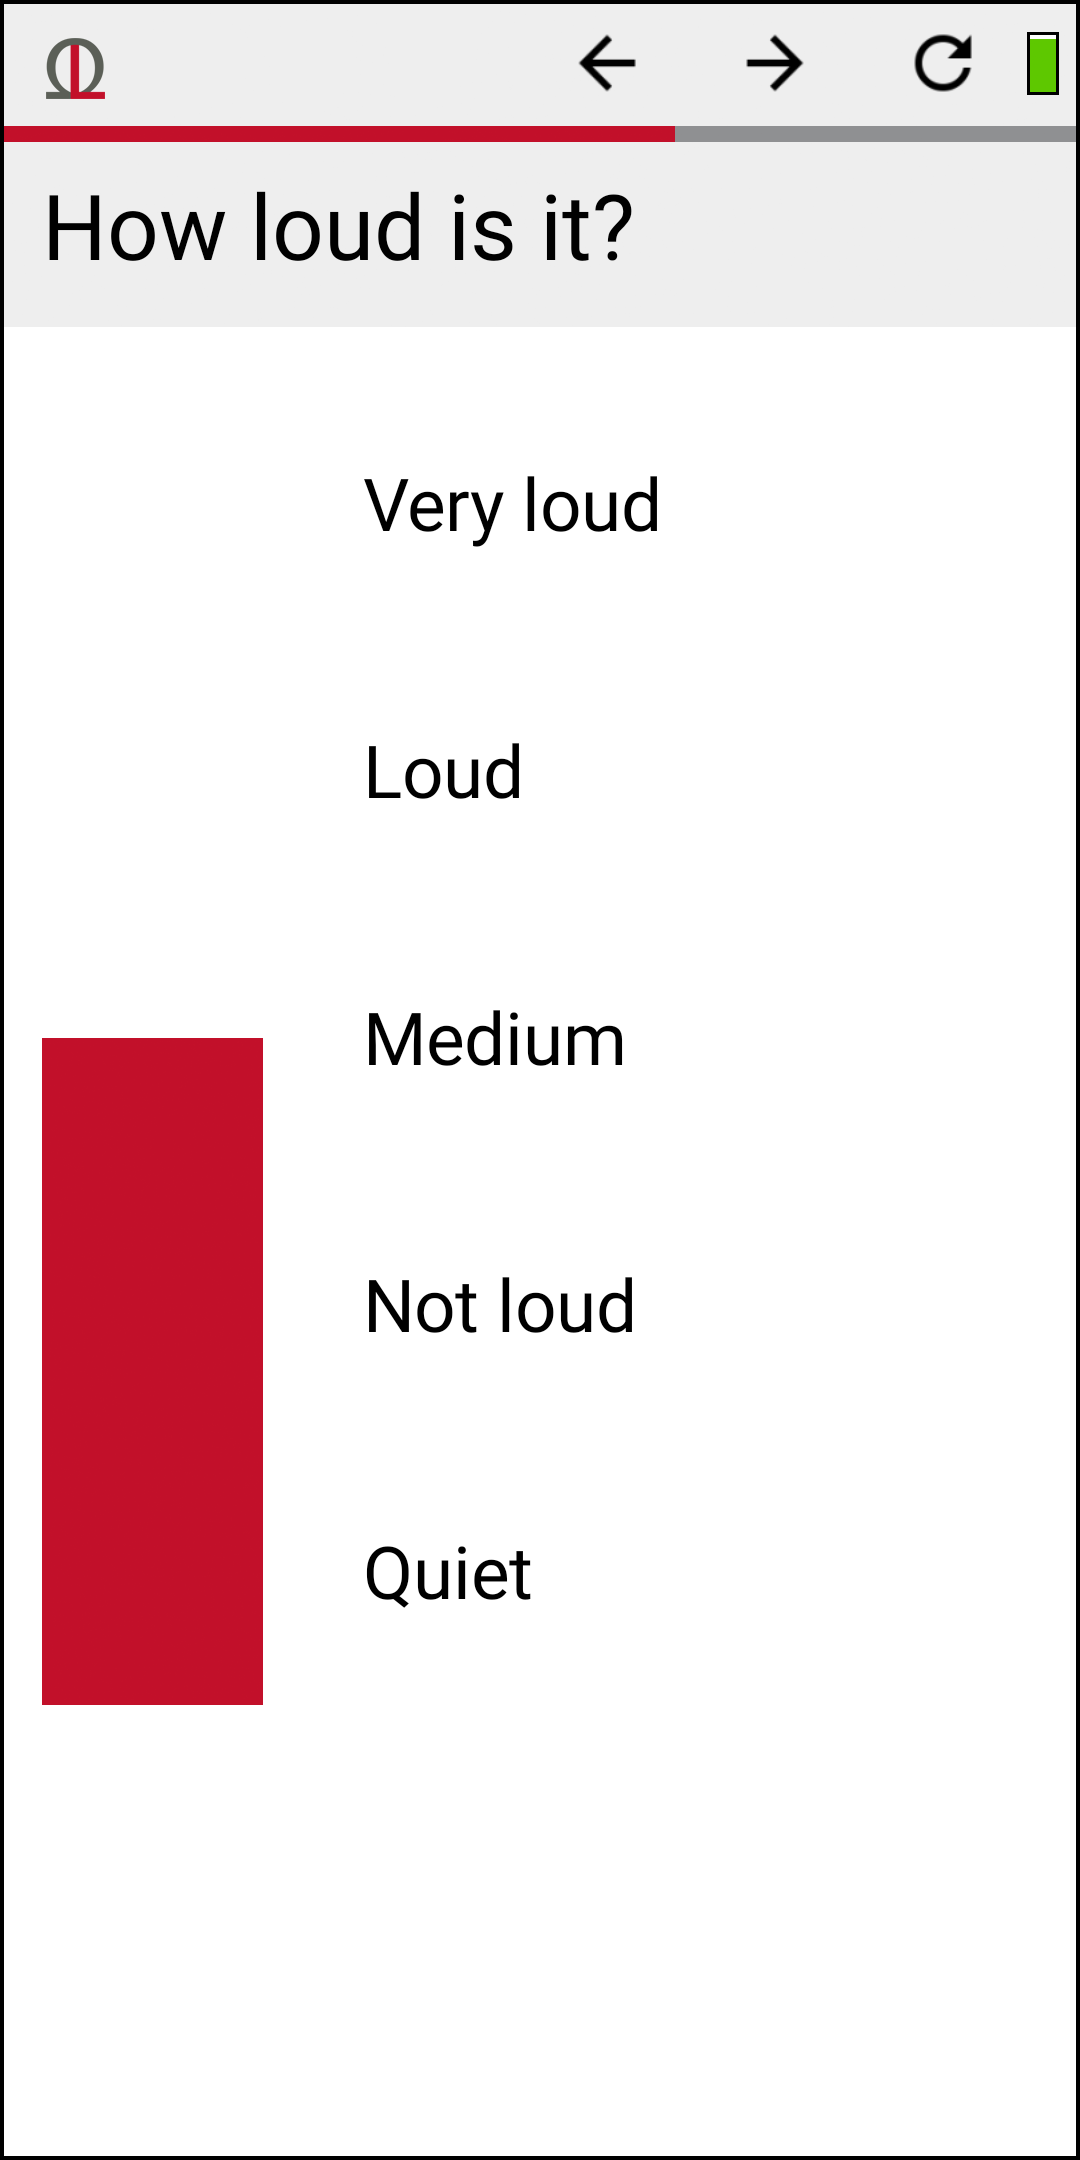
\includegraphics[width=0.30\textwidth]{images/screen_sliderfix_box.png}
		}
	\end{tabular}\\
\end{center}


\newpage


\subsubsection{Free Slider}

Free sliders are fully functional sliders which allow the user to select any value on a given scale. The result is coded as a floating point value between 0 and 1.

\begin{center}
\hspace{-1.1cm}
	\begin{tabular}{p{0.68\textwidth} p{0.25\textwidth}} 
		\raisebox{-\totalheight}{
		\begin{tcolorbox}[colback=black!10!white,colframe=black!50!white, boxsep=1pt,left=4pt,right=4pt,top=4pt,bottom=2pt]
		\texttt{\noindent
			$<$question id="10106" type="sliderFree"$>$\newline
			\hspace*{0.5cm}$<$label$>$\newline
			\hspace*{1.0cm}$<$text>How loud is it?$<$/text$>$\newline
			\hspace*{0.5cm}$<$/label$>$\newline
			\hspace*{0.5cm}$<$option id="10106\_01"$>$\newline
			\hspace*{1.0cm}$<$text$>$Very loud$<$/text$>$\newline
			\hspace*{0.5cm}$<$/option$>$\newline
			\hspace*{0.5cm}$<$option id="10106\_02"$>$\newline
			\hspace*{1.0cm}$<$text>Loud$<$/text$>$\newline
			\hspace*{0.5cm}$<$/option$>$\newline
			\hspace*{0.5cm}$<$option id="10106\_03"$>$\newline
			\hspace*{1.0cm}$<$text>Medium$<$/text$>$\newline
			\hspace*{0.5cm}$<$/option$>$\newline
			\hspace*{0.5cm}$<$option id="10106\_04"$>$\newline
			\hspace*{1.0cm}$<$text$>$Not loud$<$/text$>$\newline
			\hspace*{0.5cm}$<$/option$>$\newline
			\hspace*{0.5cm}$<$option id="10106\_05"$>$\newline
			\hspace*{1.0cm}$<$text>Quiet$<$/text$>$\newline
			\hspace*{0.5cm}$<$/option$>$\newline
			$<$/question$>$
			}
		\end{tcolorbox} 
		}
		&
		\vspace{-0.29cm}
		\raisebox{-\totalheight}{
			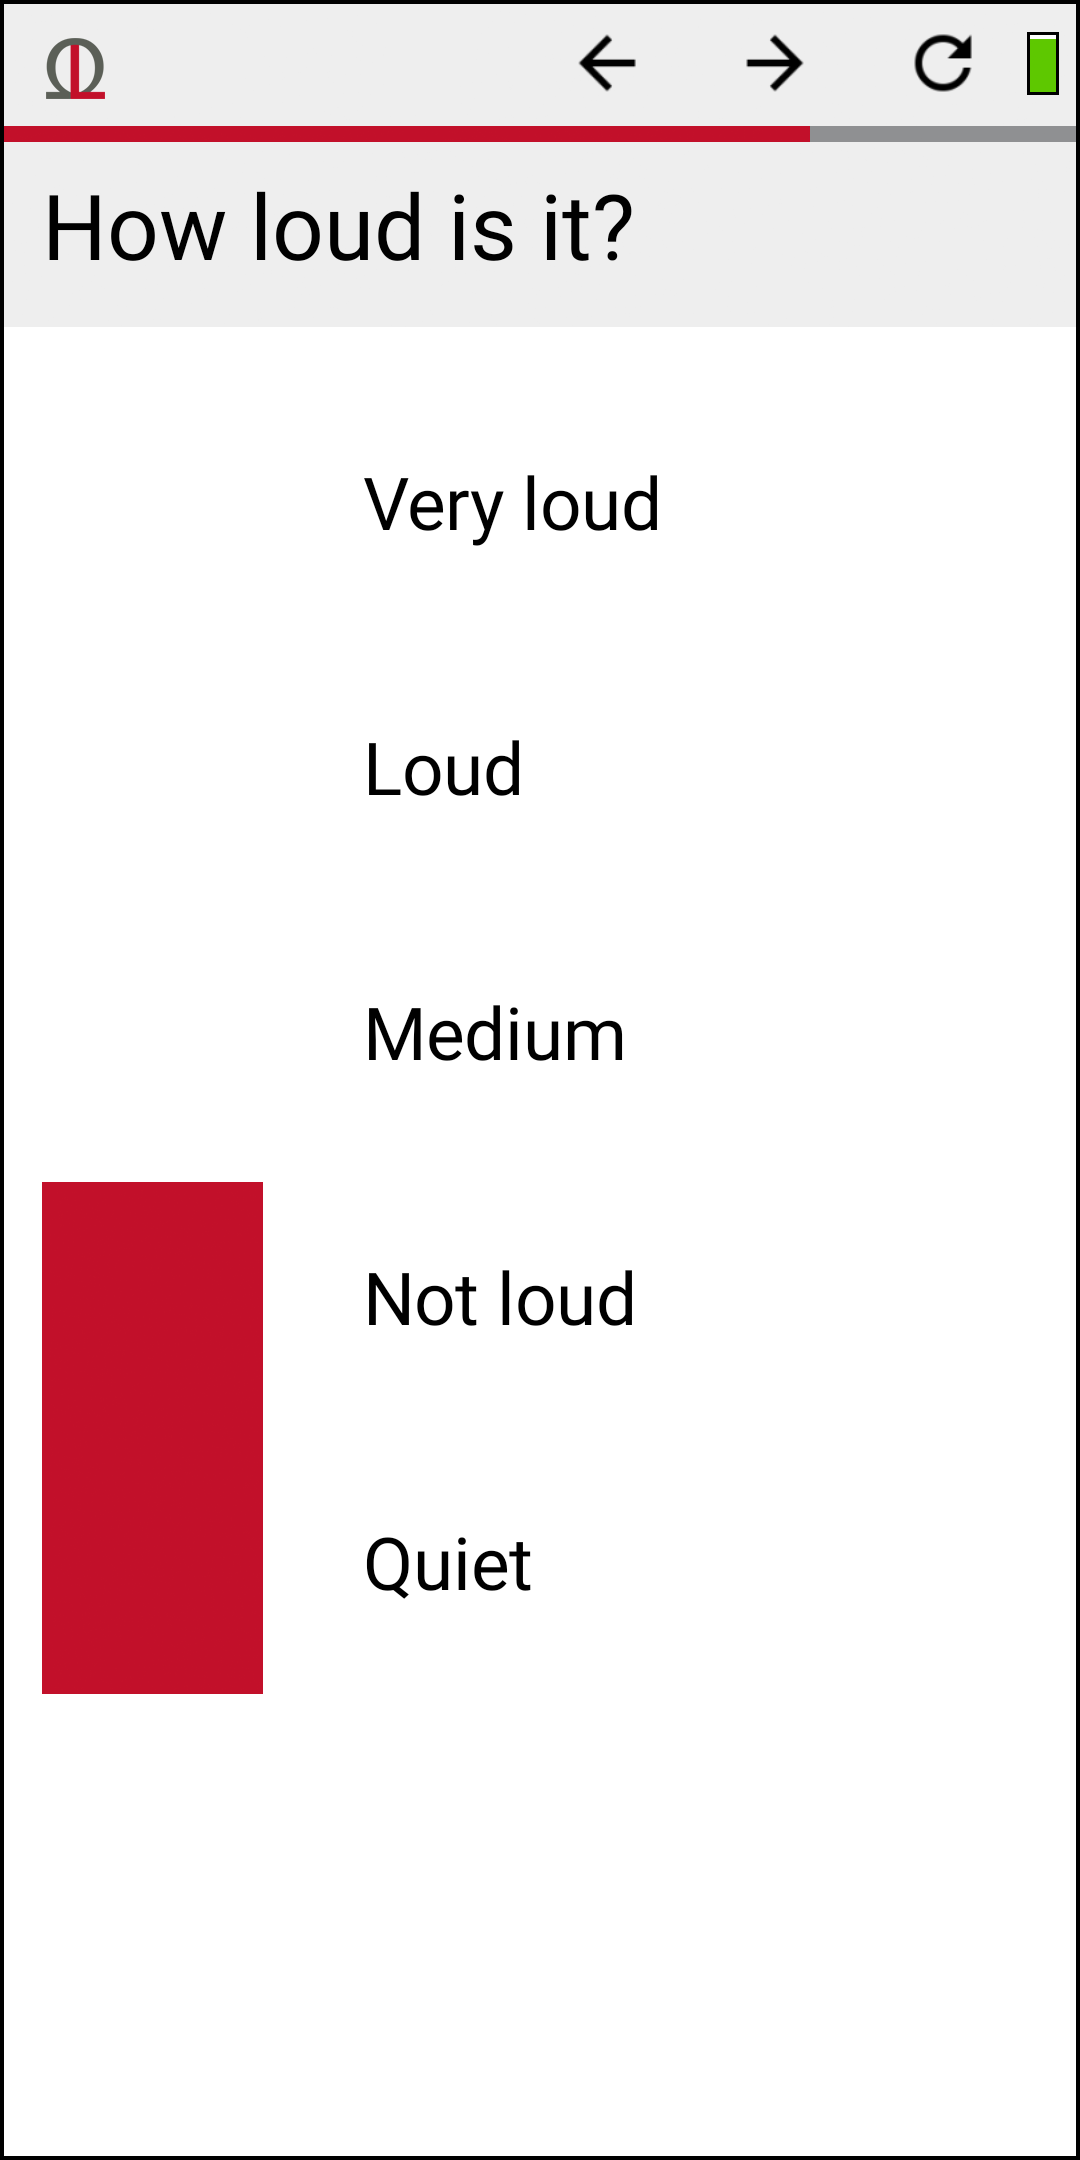
\includegraphics[width=0.30\textwidth]{images/screen_sliderfree_box.png}
		}
	\end{tabular}\\
\end{center}



\subsubsection{Time-specific behaviour}

The \emph{time} format allows for questionnaires that include aspects specific to the time of day. This question is processed internally and not displayed to the user. If the current time falls within one of the given intervals (here: 06:00-12:00 and 12:00-18:00), the corresponding id is pushed to memory and can be used as a filter for subsequent questions (consult \ref{sub:logic} for reference). This question type should therefore be placed at the beginning of a questionnaire. Use of the 24h HH:mm format is mandatory.

\begin{center}
\hspace{-0.8cm}
\begin{tabular}{p{0.68\textwidth} p{0.25\textwidth}} 
		\begin{tcolorbox}[colback=black!10!white,colframe=black!50!white, boxsep=1pt,left=4pt,right=4pt,top=4pt,bottom=2pt]
		\texttt{\noindent
			$<$question id="10109" type="time"$>$\newline
			\hspace*{0.5cm}$<$option id="10109\_01"$>$\newline
			\hspace*{1.0cm}$<$text$>$06:00-12:00$<$/text$>$\newline
			\hspace*{0.5cm}$<$/option$>$\newline
			\hspace*{0.5cm}$<$option id="10109\_02"$>$\newline
			\hspace*{1.0cm}$<$text>12:00-18:00$<$/text$>$\newline
			\hspace*{0.5cm}$<$/option$>$\newline
			$<$/question$>$
			}
		\end{tcolorbox} 
		
		&
		
	\end{tabular}\\
\end{center}


\newpage


\subsubsection{External Website}

As the name suggests, it is possible to include one or more external websites in the questionnaire, as long as internet access is provided. Two methods of calling exist. Either a website is linked without any additional information or with an identifier submitted to the server running the website. This can be helpful when the purpose of the external contents is to complete a supplementary task the results of which need to be associated with the user later. In this case a server would of course be expecting additional information of a certain format, and the term \$clientID\$ is internally replaced by the appropriate entry which is assigned via the preferences menu (\textit{Client ID}). Always ensure that the contents of the website is designed for display on a mobile device.

\begin{center}
\hspace{-1.1cm}
	\begin{tabular}{p{0.68\textwidth} p{0.25\textwidth}} 
		\raisebox{-\totalheight}{
		\begin{tcolorbox}[colback=black!10!white,colframe=black!50!white, boxsep=1pt,left=4pt,right=4pt,top=4pt,bottom=2pt]
		
		\textbf{Simple call:}\\
		
		\texttt{\noindent
			$<$question id="10107" type="website"$>$\newline
			\hspace*{0.5cm}$<$label$>$\newline
			\hspace*{1.0cm}$<$text>External Source:$<$/text$>$\newline
			\hspace*{0.5cm}$<$/label$>$\newline
			\hspace*{0.5cm}$<$option id="10107\_01"$>$\newline
      \hspace*{1.0cm}$<$text$>$https://tgm.jade-hs.de/projekte/\newline
			\hspace*{2.0cm}ihab-rl$<$/text$>$\newline
			\hspace*{0.5cm}$<$/option$>$\newline
			$<$/question$>$\\
			}
			
			\textbf{Call with parameter:}\\
		
		\texttt{\noindent
			$<$question id="10108" type="website"$>$\newline
			\hspace*{0.5cm}$<$label$>$\newline
			\hspace*{1.0cm}$<$text>External Source:$<$/text$>$\newline
			\hspace*{0.5cm}$<$/label$>$\newline
			\hspace*{0.5cm}$<$option id="10108\_01"$>$\newline
      \hspace*{1.0cm}$<$text$>$https://tgm.jade-hs.de/projekte/\newline
			\hspace*{2.0cm}ihab-rl/index.php?ClientId=\$clientID\$\newline
			\hspace*{1.0cm}$<$/text$>$\newline
			\hspace*{0.5cm}$<$/option$>$\newline
			$<$/question$>$
			}
		\end{tcolorbox} 
		}
		&
		\vspace{-0.29cm}
		\raisebox{-\totalheight}{
			
\includegraphics[width=0.3\textwidth]{images/screen_website_box.png}
		}
	\end{tabular}\\
\end{center}


\newpage


\subsubsection{Information without interaction}

There may be the need for displaying information to the user. This is where this feature comes in handy. The text in the label is displayed as a heading and the option contents is placed as free-flowing text. Similar to html, line breaks are forced by inserting $<$br/$>$. Since no behaviour is educed from this screen, an option id is not assigned.

\begin{center}
\hspace{-1.1cm}
	\begin{tabular}{p{0.68\textwidth} p{0.25\textwidth}} 
		\raisebox{-\totalheight}{
		\begin{tcolorbox}[colback=black!10!white,colframe=black!50!white, boxsep=1pt,left=4pt,right=4pt,top=4pt,bottom=2pt]
		\texttt{\noindent
			$<$question id="10110" type="infoscreen"$>$\newline
			\hspace*{0.5cm}$<$label$>$\newline
			\hspace*{1.0cm}$<$text>Title$<$/text$>$\newline
			\hspace*{0.5cm}$<$/label$>$\newline
			\hspace*{0.5cm}$<$option$>$\newline
			\hspace*{1.0cm}$<$text$>$This is some explanatory or \newline
			\hspace*{1.0cm}informational text that is displayed\newline
			\hspace*{1.0cm}to the user.$<$br/$>$It can be very long\newline
			\hspace*{1.0cm}or rather concise although we would\newline
			\hspace*{1.0cm}recommend limiting its length to one\newline 
			\hspace*{1.0cm}screen as vertical swiping might be\newline 
			\hspace*{1.0cm}confusing to the user.$<$/text$>$\newline
			\hspace*{0.5cm}$<$/option$>$\newline
			$<$/question$>$
			}
		\end{tcolorbox} 
		}
		&
		\vspace{-0.29cm}
		\raisebox{-\totalheight}{
			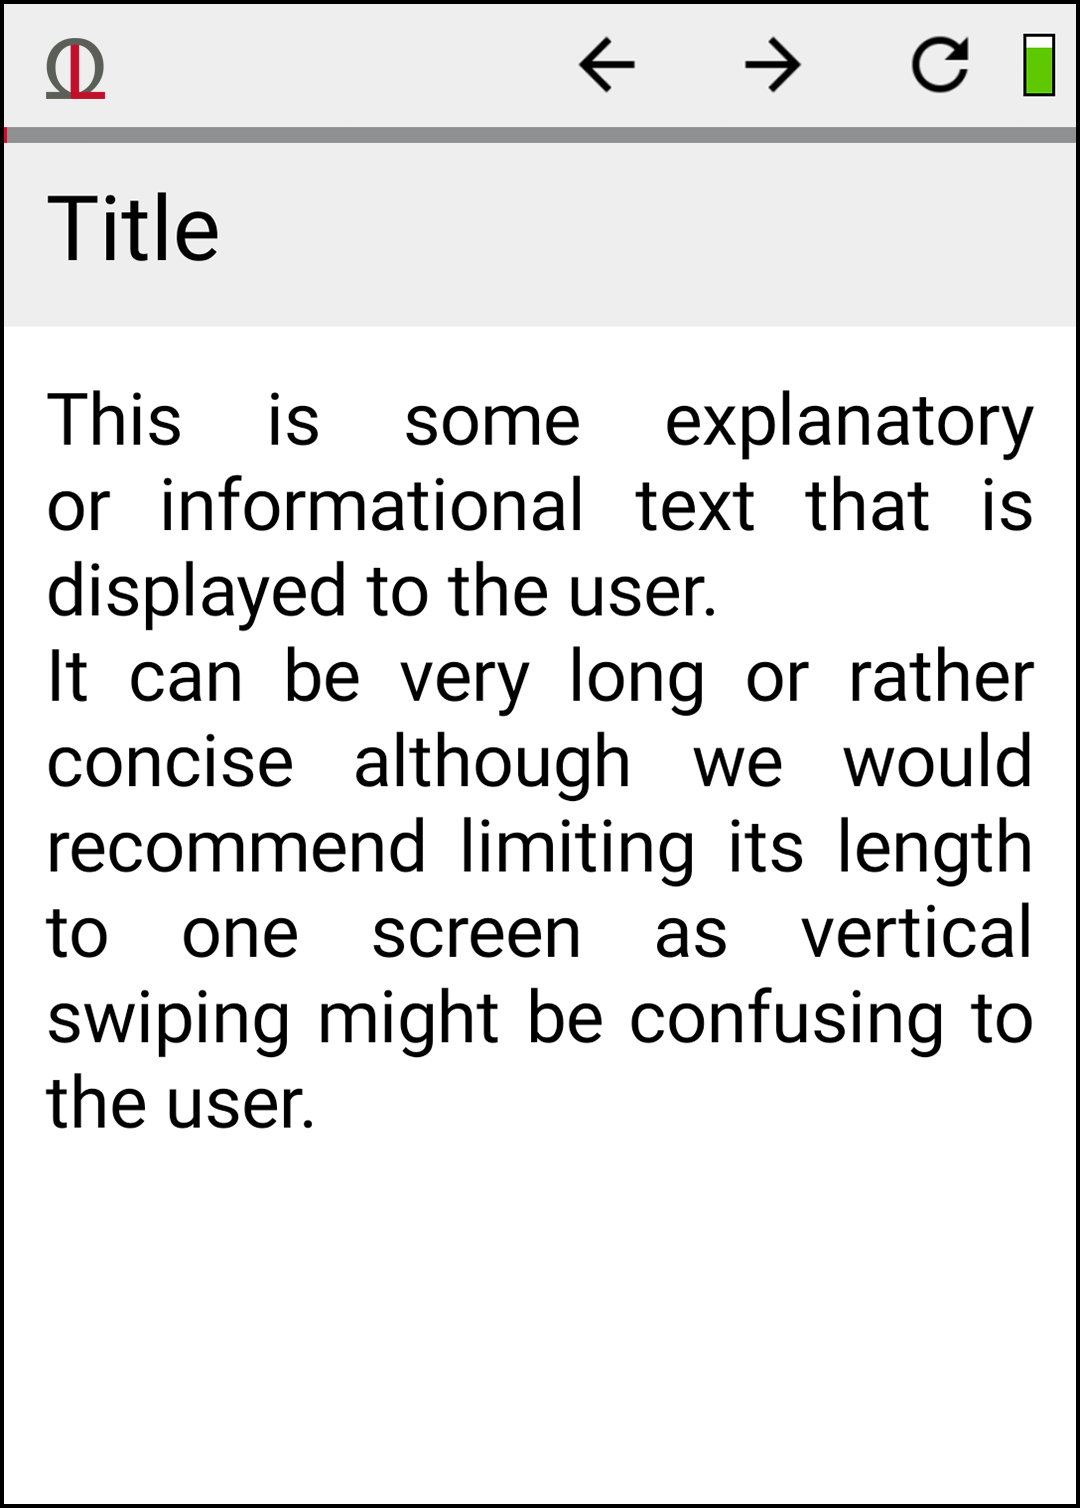
\includegraphics[width=0.30\textwidth]{images/screen_infoscreen_box.png}
		}
	\end{tabular}\\
\end{center}



\subsubsection{Information with interaction}

This is an alternative to the \emph{finish} screen, but with the option of filters. Additionally, there may exist multiple of these screens within one survey design. Pressing the button leads to completion of the questionnaire. The information text is displayed inside the heading. 

\begin{center}
\hspace{-1.1cm}
	\begin{tabular}{p{0.68\textwidth} p{0.25\textwidth}} 
		\raisebox{-\totalheight}{
		\begin{tcolorbox}[colback=black!10!white,colframe=black!50!white, boxsep=1pt,left=4pt,right=4pt,top=4pt,bottom=2pt]
		\texttt{\noindent
			$<$question id="10110" type="info"$>$\newline
			\hspace*{0.5cm}$<$label$>$\newline
			\hspace*{1.0cm}$<$text>Title$<$/text$>$\newline
			\hspace*{0.5cm}$<$/label$>$\newline
			$<$/question$>$
			}
		\end{tcolorbox}
		}
		&
		\vspace{-0.29cm}
		\raisebox{-\totalheight}{
			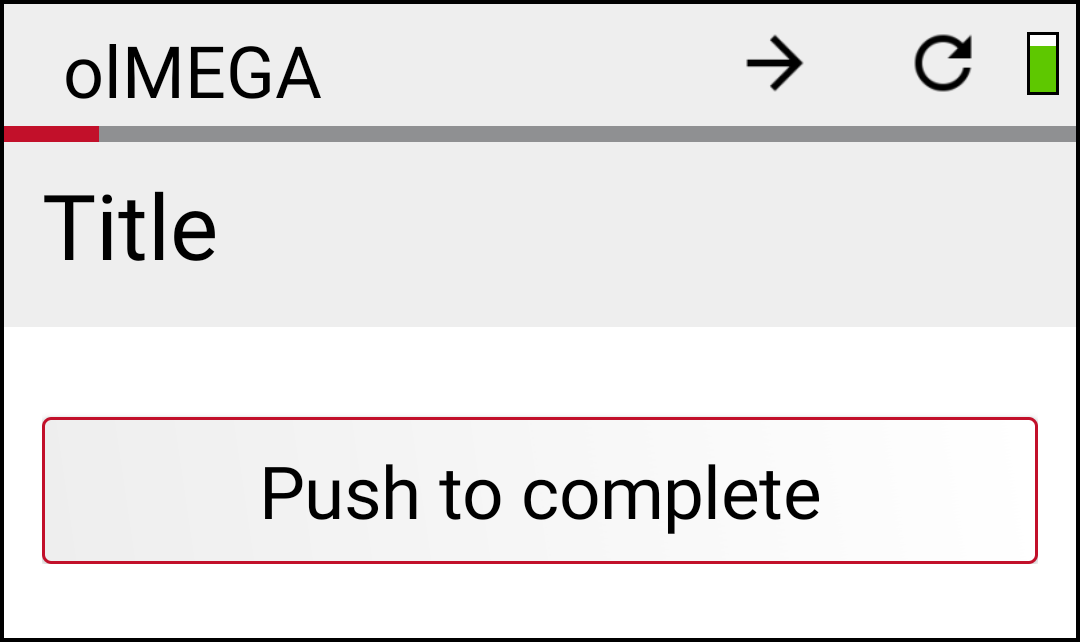
\includegraphics[width=0.30\textwidth]{images/screen_info_box.png}
		}
	\end{tabular}\\
\end{center}




\subsubsection{Finish}

The last question should be the finish page which automatically includes a button that completes the questionnaire and saves the results:

\begin{center}
\hspace{-1.1cm}
	\begin{tabular}{p{0.68\textwidth} p{0.25\textwidth}} 
		\raisebox{-\totalheight}{
			\begin{tcolorbox}[colback=black!10!white,colframe=black!50!white, boxsep=1pt,left=4pt,right=4pt,top=4pt,bottom=2pt]
				\texttt{\noindent
				$<$finish$>$\\
				\hspace*{0.5cm}$<$text$>$Thank you!$<$/text$>$\\
				$<$/finish$>$
				}
			\end{tcolorbox} 
		}
	&
		\vspace{-0.29cm}
		\raisebox{-\totalheight}{
			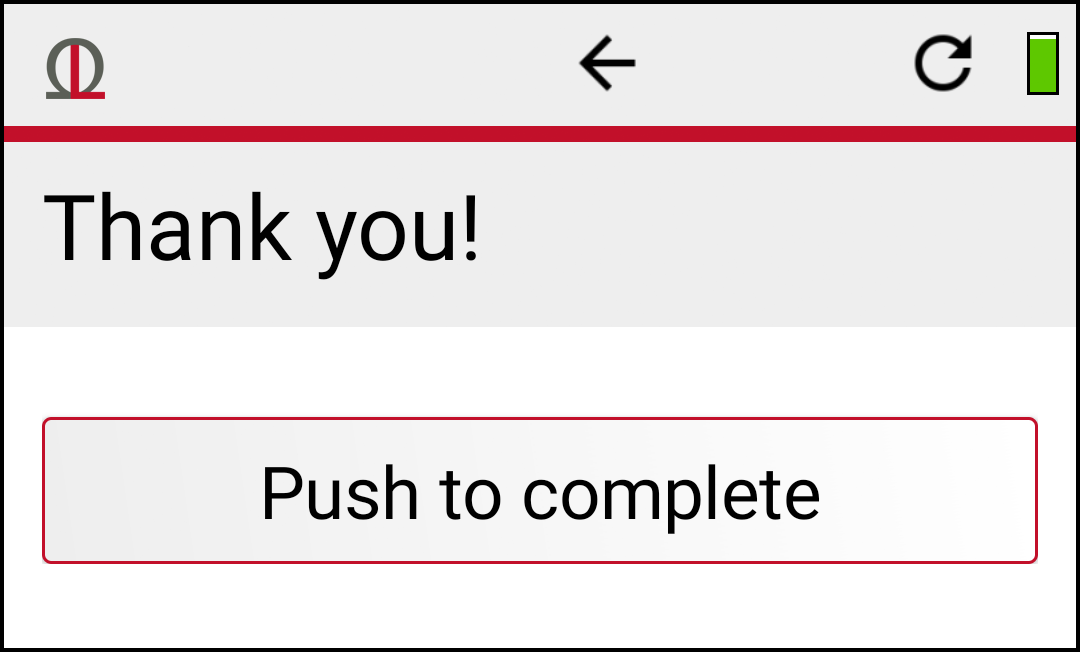
\includegraphics[width=0.30\textwidth]{images/screen_finish_crop_box.png}
		}
	\end{tabular}\\
\end{center}

\newpage

\subsection{Checkbox grouping and exclusivity}\label{subsec:goupingandexclusivity}

If only one option out of a group of options might be logically possible (see exemplary options 1-3 below), they can form a \texttt{group}. If one item out of this group is selected, the others are automatically deselected. Multiple groups can exist within one question. An extreme form of this is the \texttt{exclusive} tag (option 5), which deselects every other item from the respective list of answers except itself and automatically deselects itself if another item is chosen.

\begin{center}
	\begin{tcolorbox}[colback=black!10!white,colframe=black!50!white, boxsep=1pt,left=4pt,right=4pt,top=4pt,bottom=2pt]
		\texttt{\noindent
			$<$question id="10111" type="checkbox"$>$\\
			\hspace*{0.5cm}$<$label$>$\\
			\hspace*{1cm}$<$text$>$Where does sound originate from?$<$/text$>$\\
			\hspace*{0.5cm}$<$/label$>$\\
			\hspace*{0.5cm}$<$option id="10111\_01" group="1"$>$\\
			\hspace*{1cm}$<$text$>$Single person$<$/text$>$\\
			\hspace*{0.5cm}$<$/option$>$\\
			\hspace*{0.5cm}$<$option id="10111\_02" group="1"$>$\\
			\hspace*{1cm}$<$text$>$2-3 persons$<$/text$>$\\
			\hspace*{0.5cm}$<$/option$>$\\
			\hspace*{0.5cm}$<$option id="10111\_03" group="1"$>$\\
			\hspace*{1cm}$<$text$>$4 or more persons$<$/text$>$\\
			\hspace*{0.5cm}$<$/option$>$\\
			\hspace*{0.5cm}$<$option id="10111\_04"$>$\\
			\hspace*{1cm}$<$text$>$Public announcement$<$/text$>$\\
			\hspace*{0.5cm}$<$/option$>$\\
			\hspace*{0.5cm}$<$option id="10111\_05" condition="exclusive"$>$\\
			\hspace*{1cm}$<$text$>$It is quiet.$<$/text$>$\\
			\hspace*{0.5cm}$<$/option$>$\\
			$<$/question$>$
		}
	\end{tcolorbox}
\end{center}


\subsection{Default items}

An item can be preselected by default using the \texttt{default} tag instead of \texttt{option} as shown below. This is supported by radio buttons, checkboxes, emojis, and sliders.

\begin{center}
	\begin{tcolorbox}[colback=black!10!white,colframe=black!50!white, boxsep=1pt,left=4pt,right=4pt,top=4pt,bottom=2pt]
		\texttt{\noindent
			$<$default id="10102\_02"$>$\\
			\hspace*{0.5cm}$<$text$>$Green$<$/text$>$\\
			$<$/default$>$
		}
	\end{tcolorbox}
\end{center}


\subsection{Forced answers}

Sometimes a question might be very important and a missing answer is not an option. In this case the command \texttt{forceAnswer="true"} comes in handy. The user is unable to skip the question and after 3 attempts a dialog box with a reminding message appears on the screen.

\begin{center}
\hspace{-1.1cm}
	\begin{tabular}{p{0.68\textwidth} p{0.25\textwidth}} 
		\raisebox{-\totalheight}{
			\begin{tcolorbox}[colback=black!10!white,colframe=black!50!white, boxsep=1pt,left=4pt,right=4pt,top=4pt,bottom=2pt]
		\texttt{\noindent
			$<$question id="10101"\newline
			\hspace*{0.5cm}type="radio" \newline
			\hspace*{0.5cm}forceAnwer="true"$>$
		}
	\end{tcolorbox}
		}
	&
		\vspace{-0.29cm}
		\raisebox{-\totalheight}{
			\includegraphics[width=0.30\textwidth]{images/screen_force_box_crop.png}
		}
	\end{tabular}\\
\end{center}


\subsection{Logic}\label{sub:logic}

In order to allow for high specificity and efficiency, questions can be equipped with logical decision parameters that establish whether or not a question will be included in the current suite. The switch is located in the opening line of each question under the tag \texttt{filter} in form of a comma-separated concatenation of all included conditions.\\
\\
Two scenarios exist: positive and negative. A question will only be included if \textbf{ALL} positive conditions are satisfied and it will not be included as soon as at least \textbf{ONE} negative condition (indicated by a prefixed ``!'') is satisfied (e.g. \texttt{filter="10103\_02,10103\_05,!10111\_09"}).\\ 
\\
$\rightarrow$ Think: positive - necessary criterion, negative -- sufficient criterion.\\
\\
The filter conditions are the option ID's of answer items from earlier questions of the current session. Whenever an answer is chosen by the user, its ID is stored in memory and before a question is displayed, a filter checks whether given conditional ID's are present in the memory.\\

\begin{center}
	\begin{tcolorbox}[colback=black!10!white,colframe=black!50!white, boxsep=1pt,left=4pt,right=4pt,top=4pt,bottom=2pt]
		\texttt{\noindent
			$<$question id="10112" type="radio" filter="10103\_02,10103\_05,!10111\_09"$>$
		}
	\end{tcolorbox}
\end{center}

Note that entries can be spread across multiple lines in order to increase readability.

\begin{center}
	\begin{tcolorbox}[colback=black!10!white,colframe=black!50!white, boxsep=1pt,left=4pt,right=4pt,top=4pt,bottom=2pt]
		\texttt{\noindent
			$<$question id="10112"\newline
			\hspace*{0.5cm}type="radio" \newline
			\hspace*{0.5cm}filter="10103\_02,\newline
			\hspace*{1.0cm}10103\_05,\newline
			\hspace*{1.0cm}!10111\_09"$>$
		}
	\end{tcolorbox}
\end{center}


\subsection{Comments}

Two types of comments are supported by the questionnaire format. Single line comments start with ``//'', comments spread across multiple lines are parenthesized by ``\texttt{$/*$}'' and ``\texttt{$*/$}''.

\begin{center}
	\begin{tcolorbox}[colback=black!10!white,colframe=black!50!white, boxsep=1pt,left=4pt,right=4pt,top=4pt,bottom=2pt]
		\texttt{\noindent
			// One line comment\newline
			\newline
			/* Here is a\newline
			slightly longer\newline
			comment */
		}
	\end{tcolorbox}
\end{center}


\newpage

\section{Error Messages}

\begin{wrapfigure}{r}{5cm}
\vspace{-0.5cm}
		\centering
			\begin{minipage}{0.30\textwidth}
			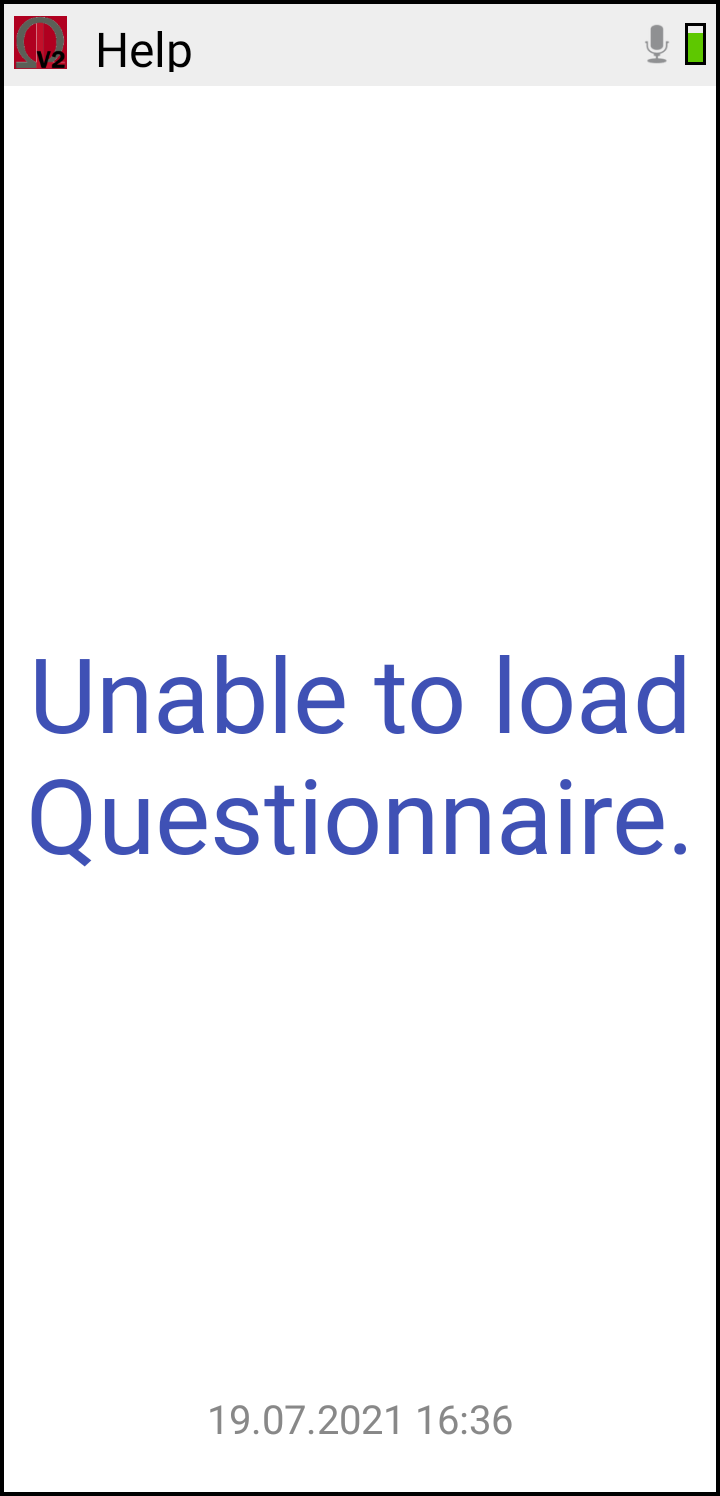
\includegraphics[width=1.00\textwidth]{images/screen_error_quest.png}
			\label{fig:menu}
			\end{minipage}
	\end{wrapfigure}

Inside the application there exist 6 different error messages. These are displayed on the main screen in case of malfunction or general situations that require the user's attention.\\
\\
\textbf{No Input Profile Config selected:} The application needs some information on whether it should extract features and - if so - which audio source is desired. Please select an operation mode via the in-app preferences under \texttt{Operation Mode}. See also \ref{sub:operationmode} for more information. \\
\\
\textbf{Stage Manager Config-File [*] not valid:} The selected operation mode [*].xml file is invalid. Please check the file you are using.\\
\\
\textbf{Unable to start Kiosk-Mode -- Please check DeviceOwner Setting:} The KIOSK mode relies on 2 prerequisites. A device owner must be initiated (see \ref{sub:installation} for reference), and the ``Experimenter'' setting must be unset.\\
\\
\textbf{Please charge the smartphone:} Strictly speaking this is not an error but a suggestion to do exactly that. This message is shown when the battery level falls below 10\%. The device will probably work for 30 more minutes but, if possible, should be recharged soon.\\
\\
\textbf{Battery level critical - application stopped:} Battery level is below 5\% and the connection was cut. In order to protect the device and prevent data loss, it should be connected to a charger immediately.\\
\\
\textbf{Unable to load questionnaire:} No questionnaire .xml file could be found in the corresponding folder on the mobile device (\texttt{sdcard/olmega/quest}). Please upload a file and restart the application. If the error still prevails, please access the in-app preferences and select it manually (\emph{Select questionnaire} at the top of the preferences menu). Then restart the application. If you are using an older version of the system (titled \emph{IHAB}), the correct directory to upload to is (\texttt{sdcard/ihab/quest}).

\clearpage

\section{Resulting file}

Completing a questionnaire results in an .xml file being generated in the \texttt{data} folder. The file name is composed of the Device ID, the current date in \texttt{yyyyMMdd} (year, month, day) and the time of completion in \texttt{HHmmssSSS} (24h hours, minutes, seconds, milliseconds), for example \texttt{cbaaacf404279a80\_20200430\_125224699.xml}.\\
\\
The file contains information on whether the questionnaire was taken upon a reminder or deliberately (\texttt{motivation}: auto/manual), which questionnaire design it was based on, the Device ID, version of the application, start and end dates as well as the provided answers.

\begin{center}
	\begin{tcolorbox}[colback=black!10!white,colframe=black!50!white, boxsep=1pt,left=4pt,right=4pt,top=4pt,bottom=2pt]
		\texttt{\noindent
			$<$?xml version="1.0" encoding="utf-8"?$>$\newline
			$<$mobiquest$>$\newline
			$<$motivation motivation ="manual"/$>$\newline
			$<$record uri="tmp/cbaaacf404279a80\_20200430\_125224699.xml"\newline
			\hspace*{0.5cm}survey\_uri="tmp.xml"$>$\newline
			$<$value device\_id="cbaaacf404279a80"/$>$\newline
			$<$value start\_date="2020-04-30T12:52:24"/$>$\newline
			$<$value start\_date\_UTC="2020-04-30T12:52:24"/$>$\newline
			$<$value app\_version="1.5"/$>$\newline
			$<$value question\_id="10101" option\_ids="1010102"/$>$\newline
			$<$value question\_id="10102" option\_ids="1010202"/$>$\newline
			$<$value question\_id="10103" option\_ids="1010301"/$>$\newline
			$<$value question\_id="10104" option\_ids="Some generic text."/$>$\newline
			$<$value question\_id="10105" option\_ids="1010504"/$>$\newline
			$<$value question\_id="10106" option\_ids="0.36958176"/$>$\newline
			$<$value question\_id="10107"/$>$\newline
			$<$value end\_date="2020-04-30T12:53:13"/$>$\newline
			$<$value end\_date\_UTC="2020-04-30T12:53:13"/$>$\newline
			$<$/record$>$\newline
			$<$/mobiquest$>$
		}
	\end{tcolorbox}
\end{center}


\clearpage


\section{Objective data}

Additional to the facilitation of questionnaires, the olMEGA application also offers real-time extraction of acoustic features, based on the operation mode (see \ref{sub:operationmode}). These features are namely \emph{RMS Level}, \emph{Zero-Crossing-Rate} (ZCR), and \emph{Power Spectral Density} (PSD) and they are stored in chunks of a size that can be edited inside the preferences menu (usually a length of 60\,s). Although we recommend data extraction and interpretation using our Matlab interface (see \ref{sec:transfer}), here is some information on the file structure, which holds true for every feature. Each file contains a header which is holding basic information e.g. time stamps, sampling rate, dimensions, and logistics like frame length or hop size. The header is followed by a series of data packages that follow the structure depicted below.\\

\textbf{Header:}

\begin{center}
	\begin{tcolorbox}[colback=black!10!white,colframe=black!50!white, boxsep=1pt,left=4pt,right=4pt,top=4pt,bottom=2pt]
	\texttt{
		\begin{tabularx}{\textwidth}{l|l|X} 
			Type & \# & Contents\\
			\hline
			int32 & 1 & \# frames in current chunk\\
			int32 & 1 & \# dimensions (including frame time stamps)\\
			int32 & 1 & block size in samples\\
			int32 & 1 & hop size in samples\\  
			int32 & 1 & audio sampling rate\\
			byte & 16 & time stamp of block (yyyyMMdd\_HHmmssSSS)\\
		\end{tabularx}
		}
	\end{tcolorbox}
\end{center}

\textbf{Data:}

\begin{center}
	\begin{tcolorbox}[colback=black!10!white,colframe=black!50!white, boxsep=1pt,left=4pt,right=4pt,top=4pt,bottom=2pt]
	\texttt{
		\begin{tabularx}{\textwidth}{l|l|X} 
			Type & \# & Contents\\
			\hline
			double & N & block time + data\\
		\end{tabularx}
		}
	\end{tcolorbox}
\end{center}

N is the number of dimensions including timestamps times the number of blocks or frames inside a chunk. Times and feature data are concatenated as follows with block times respectively denoting beginning and end of a block:\\

\begin{tcolorbox}[colback=black!10!white,colframe=black!50!white, boxsep=1pt,left=4pt,right=4pt,top=4pt,bottom=2pt]
	\texttt{
		[ blocktime(1) blocktime(2) feature(1) feature(2) ... feature(L-2)\\
		\color{black!10!white}[\ \ \color{black} blocktime(2) blocktime(3) feature(1) feature(2) ... feature(L-2) ]
	}
\end{tcolorbox}
\vspace{0.5cm}
with L being the block size in samples and the data formatted as big endian.


\clearpage


\section{Data Extractor}\label{sec:transfer}

For every questionnaire that has been answered, a resulting .xml file is produced which can be found in the \textit{data} folder within the application directory. Acoustical feature data is placed in the \textit{features} folder. In order to simplify as well as secure data transfer we have developed a Matlab interface which can also be used to control some functions of the smartphone. The software can be downloaded from GitHub: \url{https://github.com/ol-MEGA/olMEGA_DataExtraction.git}. Please note that so far it has only been tested under Windows 7/10. Figure \ref{fig:DataExtractor} shows the main application screen.\\
\\
The application is divided into 6 tabs:

\begin{itemize}[label=\ClrSquare{jadeRed}]
	\item \textbf{Statistics:} This tab displays the number of feature and questionnaire result files found in the user directory. It also yields information on whether or not a log file is present.
	\item \textbf{User data:} Here is where a new user account is created or an existing user directory is loaded.
	\item \textbf{Activity:} After loading a directory this tab displays an overview graphic of all the gathered data. More information on this graphic is given in \ref{sub:activity}.
	\item \textbf{Output:} Information about the current task or contents of a directory is displayed here.
	\item \textbf{Navigation:} Once the Activity panel shows the overview graphic, these tools enable the user to navigate through the data.
	\item \textbf{Phone actions:} These options control the mobile device. There is the option of transferring data from the smartphone to the computer, to erase all experiment data from the phone, kill the mobile application, and reboot the device.
\end{itemize}

\begin{figure}[h]
	\centering
		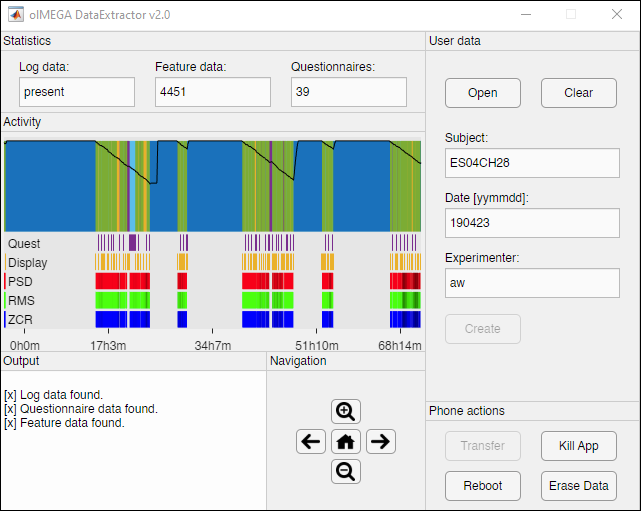
\includegraphics[width=0.90\textwidth]{images/DataExtractor.png}
	\caption{Data Extractor: Main Screen}
	\label{fig:DataExtractor}
\end{figure}



\subsection{The Activity panel}\label{sub:activity}


The graphic overview consists of the main technical parameters that were recorded during the experiment run. The top half shows the state that the mobile application was in at a given time -- one distinct colour for each state. Printed in black is the battery status over the run of the experiment. On clicking into the graphic, a legend appears which relates the colours to states, along with their numeric proportions (Figure \ref{fig:Legend}). 

\begin{itemize}
	\item [\ClrSquareBig{ml_charging}] \textbf{Charging:} The phone is charging and no data is recorded.
	\item [\ClrSquareBig{ml_error}] \textbf{Error:} There exists a significant error. No data is recorded.
	\item [\ClrSquareBig{ml_proposing}] \textbf{Proposing:} An alarm is set off and the user is encouraged to conduct a survey.
	\item [\ClrSquareBig{ml_connecting}] \textbf{Connecting:} The smartphone is trying to establish a connection to the transmitter.
	\item [\ClrSquareBig{ml_running}] \textbf{Running:} The application is running without any errors.
	\item [\ClrSquareBig{ml_quest}] \textbf{Quest:} A questionnaire is taken.
	\item [\ClrSquareBig{ml_offline}] \textbf{Offline:} The application is closed.
\end{itemize}

 The lower half of the graphic consists of multiple illustrations: The uppermost, aubergine-coloured plot displays all the time a questionnaire was open. Second are the times the display of the smartphone was illuminated. This information is printed in orange. The lower three plots show the existence and quality of extracted acoustical features, PSD, RMS, and zero-crossing rate. The shading of their colour represents the percentage of error found in the data (the darker, the more errors). These errors can be: too loud, too quiet, signal is mono, and invalid coherence, meaning that the miniature microphones were most likely not head-worn at the time. All error thresholds are motivated by experience and might be adjusted in the future.

\begin{figure}
	\centering
		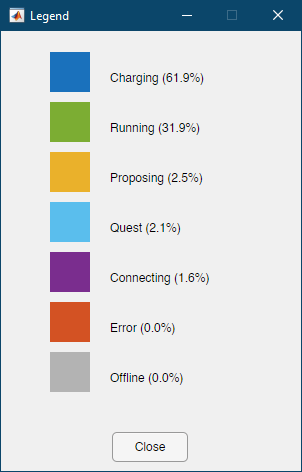
\includegraphics[width=0.30\textwidth]{images/Legend.PNG}
	\caption{Data Extractor: Legend}
	\label{fig:Legend}
\end{figure}




\subsection{Transferring data from the smartphone to the computer}\label{sub:transfer}


\begin{enumerate}
	\item Connect the phone to the computer
	\item Enter \textit{Subject} name. The entry form allows any combination of letters and numbers, but is limited to 8 characters.
	\item Enter \textit{Date} in the given format [yymmdd].
	\item Enter \textit{Experimenter} token. This is limited to a combination of 2 characters.
	\item Now click \textit{Create}.
	\item A dialog box will appear which lets you specify the directory in which a new subject folder is created.
	\item Now click the button labeled \textit{Transfer}.
	\item In some cases an error dialog appears, warning either about too many devices connected or no devices found. Simply click \textit{OK} and select \textit{Transfer} again.
	\item After the transfer process has finished, the overview graphic (see \ref{sub:activity}) is calculated and presented in the \textit{Activity} tab.
\end{enumerate}




\clearpage


\section{License}

 Copyright 2020 \Institute\\
\\
   Licensed under the Apache License, Version 2.0 (the ``License'');
   you may not use this file except in compliance with the License.
   You may obtain a copy of the License at\\
\\
	 \url{http://www.apache.org/licenses/LICENSE-2.0}\\
\\
   Unless required by applicable law or agreed to in writing, software
   distributed under the License is distributed on an ``AS IS'' BASIS,
   WITHOUT WARRANTIES OR CONDITIONS OF ANY KIND, either express or implied.
   See the License for the specific language governing permissions and
   limitations under the License.

\end{document} 